% !TeX program = xelatex

% ============================================================================
% HƯỚNG DẪN VÀ BẢN ĐỒ TỆP
% ============================================================================
% Bộ báo cáo chỉ gồm main.tex và images/ chứa hình ảnh.
% Overleaf: Settings > Compiler > XeLaTeX; Main document = main.tex.
% Biên dịch lại từ đầu sau khi đổi compiler; không dùng pdfLaTeX.
% Tìm các tiêu đề đánh số dưới đây để di chuyển giữa từng thành phần.
% 01 Gói thư viện | 02 Font | 03 Thông tin | 04 Định dạng
% 05 Lệnh bổ trợ | 06 Bắt đầu | 07 Bìa và phần đầu
% 08–13 Sáu chương | 14 Tài liệu tham khảo

% ============================================================================
% 01. KHAI BÁO TÀI LIỆU VÀ GÓI THƯ VIỆN
% ============================================================================

\RequirePackage{fix-cm}
\documentclass[12pt,a4paper]{article}
\usepackage{iftex}
\ifPDFTeX
  \PackageError{tdtu-report}{Select XeLaTeX}{Times New Roman requires fontspec.}
  \expandafter\stop
\fi
\usepackage{fontspec,geometry}
\usepackage{amsmath,amssymb,graphicx,float,booktabs,array,tabularx,longtable}
\usepackage{xcolor,tikz,caption,indentfirst,setspace,fancyhdr,etoolbox}
\usepackage{titlesec,tocloft,xurl}
\usepackage[unicode,hidelinks]{hyperref}

% ============================================================================
% 02. PHÔNG CHỮ
% ============================================================================
% ============================================================================
% PHÔNG CHỮ — giữ Times New Roman; không thay bằng phông mô phỏng
% ============================================================================
\IfFontExistsTF{Times New Roman}{%
  \setmainfont{Times New Roman}%
}{%
  \PackageError{tdtu-report}{Times New Roman is required}{Install Times New Roman in the compilation environment. Select XeLaTeX on Overleaf.}%
}
% KẾT THÚC: 02. PHÔNG CHỮ


% ============================================================================
% 03. THÔNG TIN ĐỀ TÀI, TÁC GIẢ VÀ GIẢNG VIÊN
% ============================================================================
% Thông tin hiện có của báo cáo; không thay đổi nội dung học thuật.
\newcommand{\TenDeTai}{Phân loại nội dung đa phương thức zero-shot bằng mô hình thị giác--ngôn ngữ}
\newcommand{\NgayBaoCao}{ngày 16 tháng 11 năm 2026}
\newcommand{\UniversityOwner}{TỔNG LIÊN ĐOÀN LAO ĐỘNG VIỆT NAM}
\newcommand{\UniversityName}{TRƯỜNG ĐẠI HỌC TÔN ĐỨC THẮNG}
\newcommand{\FacultyName}{KHOA CÔNG NGHỆ THÔNG TIN}
\newcommand{\ProjectTitle}{PHÂN LOẠI NỘI DUNG ĐA PHƯƠNG\\THỨC ZERO-SHOT BẰNG MÔ HÌNH\\THỊ GIÁC--NGÔN NGỮ}
\newcommand{\ReportType}{BÁO CÁO CUỐI KỲ}
\newcommand{\CourseName}{DỰ ÁN CÔNG NGHỆ THÔNG TIN}
\newcommand{\StudentOne}{LÊ VĂN DUY -- 52300102}
\newcommand{\StudentTwo}{NGUYỄN MẠNH HÙNG -- 52300107}
\newcommand{\SupervisorName}{TS. Lương Thị Ngọc Khánh}
\newcommand{\ReportCity}{THÀNH PHỐ HỒ CHÍ MINH}
\newcommand{\ReportYear}{2026}
\newcommand{\SignatureDate}{TP. Hồ Chí Minh, \NgayBaoCao}
\newcommand{\SignatureName}{Lê Văn Duy\hfill Nguyễn Mạnh Hùng}
\newcommand{\UniversityLogo}{images/tdtu_template_logo.png}

% KẾT THÚC: 03. THÔNG TIN ĐỀ TÀI, TÁC GIẢ VÀ GIẢNG VIÊN


% ============================================================================
% 04. QUY TẮC ĐỊNH DẠNG VÀ TỌA ĐỘ BÌA
% ============================================================================
% ============================================================================
% CẤU HÌNH BỐ CỤC — kích thước, lề, giãn dòng, tiêu đề và danh mục
% ============================================================================
% 1. CỠ CHỮ: theo yêu cầu người dùng; không dùng \large/\LARGE tương đối.
\newcommand{\BodySize}{13}
\newcommand{\BodyLeading}{15.6}
\newcommand{\BodyLineStretch}{1.5}
\newcommand{\CoverSize}{14}
\newcommand{\CoverProjectSize}{24}
\newcommand{\CoverReportSize}{22}
\newcommand{\HeadingSize}{16}
\newcommand{\SubheadingSize}{14}
\newcommand{\CoverFont}{\fontsize{\CoverSize}{18}\selectfont}
\newcommand{\CoverProjectFont}{\fontsize{\CoverProjectSize}{30}\selectfont}
\newcommand{\CoverReportFont}{\fontsize{\CoverReportSize}{28}\selectfont}
\newcommand{\HeadingFont}{\fontsize{\HeadingSize}{24}\selectfont}
\newcommand{\SubheadingFont}{\fontsize{\SubheadingSize}{21}\selectfont}
\newcommand{\BodyFont}{\fontsize{\BodySize}{\BodyLeading}\selectfont}

% 2. GIẤY/LỀ: từ sectPr của template_report.docx.
\geometry{a4paper,top=3.5cm,bottom=3cm,left=3.5cm,right=2cm,headheight=18pt,headsep=1cm}
\setlength{\parindent}{1.27cm}
\setlength{\parskip}{0pt}
\setlength{\emergencystretch}{2em}
\widowpenalty=10000
\clubpenalty=10000
\raggedbottom
% normalsize phải là 13 pt kể cả sau titlepage, bảng, danh mục hoặc nhóm lệnh.
\makeatletter
\renewcommand\normalsize{\@setfontsize\normalsize{\BodySize pt}{\BodyLeading pt}}
\makeatother
\normalsize

% 3. NHÃN TIẾNG VIỆT VÀ SỐ TRANG: không có số trên bìa; Roman/Arabic ở main.tex.
\renewcommand{\contentsname}{MỤC LỤC}
\renewcommand{\listfigurename}{DANH MỤC HÌNH VẼ}
\renewcommand{\listtablename}{DANH MỤC BẢNG BIỂU}
\renewcommand{\figurename}{Hình}
\renewcommand{\tablename}{Bảng}
\pagestyle{fancy}\fancyhf{}
\fancyhead[C]{\BodyFont\thepage}
\renewcommand{\headrulewidth}{0pt}
\fancypagestyle{plain}{\fancyhf{}\fancyhead[C]{\BodyFont\thepage}\renewcommand{\headrulewidth}{0pt}}

% 4. CHƯƠNG/MỤC: chương 16 pt; các cấp mục 14 pt; giữ thụt đầu đoạn sau tiêu đề.
\titleformat{\section}{\HeadingFont\bfseries}{CHƯƠNG \thesection.}{0.6em}{}
\titleformat{\subsection}{\SubheadingFont\bfseries}{\thesubsection}{0.6em}{}
\titleformat{\subsubsection}{\SubheadingFont\bfseries\itshape}{\thesubsubsection}{0.6em}{}
\titleformat{\paragraph}[block]{\SubheadingFont\itshape}{}{0pt}{}
\titlespacing{\section}{0pt}{0pt}{12pt}
\titlespacing{\subsection}{0pt}{12pt}{6pt}
\titlespacing{\subsubsection}{0pt}{10pt}{6pt}
\titlespacing{\paragraph}{0pt}{8pt}{6pt}
\setcounter{secnumdepth}{3}
\setcounter{tocdepth}{3}
\newcommand{\Chapter}[1]{\clearpage\section{#1}}

% 5. PHẦN ĐẦU: dạng * không đưa vào mục lục, như mẫu DOCX.
\makeatletter
\newcommand{\RestoreParagraphIndent}{\par\@afterindenttrue\@afterheading}
\NewDocumentCommand{\FrontHeading}{s m}{%
  \clearpage\phantomsection
  \IfBooleanF{#1}{\addcontentsline{toc}{section}{#2}}%
  \begin{center}\HeadingFont\bfseries #2\end{center}%
  \par\nobreak\vspace{6pt}\@afterindenttrue\@afterheading
}
% Tóm tắt: tên đề tài ở trên tiêu đề, theo DOCX mẫu mới được yêu cầu.
\newcommand{\SummaryHeading}[2]{%
  \clearpage\phantomsection
  \begin{center}\HeadingFont\bfseries #1\par\vspace{6pt}#2\end{center}%
  \par\nobreak\vspace{6pt}\@afterindenttrue\@afterheading
}
\makeatother

% 6. MỤC LỤC VÀ DANH MỤC: tiêu đề 16 pt, toàn bộ mục và số trang 13 pt.
\renewcommand{\cfttoctitlefont}{\hfill\HeadingFont\bfseries}
\renewcommand{\cftaftertoctitle}{\hfill}
\renewcommand{\cftloftitlefont}{\hfill\HeadingFont\bfseries}
\renewcommand{\cftafterloftitle}{\hfill}
\renewcommand{\cftlottitlefont}{\hfill\HeadingFont\bfseries}
\renewcommand{\cftafterlottitle}{\hfill}
\renewcommand{\cftsecfont}{\BodyFont\bfseries}
\renewcommand{\cftsecpagefont}{\BodyFont\bfseries}
\renewcommand{\cftsubsecfont}{\BodyFont}
\renewcommand{\cftsubsecpagefont}{\BodyFont}
\renewcommand{\cftsubsubsecfont}{\BodyFont}
\renewcommand{\cftsubsubsecpagefont}{\BodyFont}
\renewcommand{\cftfigfont}{\BodyFont}
\renewcommand{\cftfigpagefont}{\BodyFont}
\renewcommand{\cfttabfont}{\BodyFont}
\renewcommand{\cfttabpagefont}{\BodyFont}
\renewcommand{\cftsecpresnum}{CHƯƠNG }
\renewcommand{\cftsecaftersnum}{.}
\setlength{\cftsecnumwidth}{2.8cm}
\renewcommand{\cftsecleader}{\cftdotfill{\cftdotsep}}
\setlength{\cftsubsecindent}{0.75cm}
\setlength{\cftsubsecnumwidth}{1.1cm}
\setlength{\cftsubsubsecindent}{1.5cm}
\setlength{\cftsubsubsecnumwidth}{1.5cm}
\renewcommand{\cftfigpresnum}{Hình }
\renewcommand{\cftfigaftersnum}{: }
\setlength{\cftfignumwidth}{2.4cm}
\renewcommand{\cfttabpresnum}{Bảng }
\renewcommand{\cfttabaftersnum}{: }
\setlength{\cfttabnumwidth}{2.4cm}

% 7. HÌNH/BẢNG/CÔNG THỨC: số tự động theo chương, nội dung/caption 13 pt.
\numberwithin{figure}{section}
\numberwithin{table}{section}
\numberwithin{equation}{section}
\graphicspath{{images/}}
\DeclareCaptionFont{tdtubody}{\BodyFont}
\captionsetup{font=tdtubody,labelfont=normalfont,labelsep=colon,justification=centering}
\newcommand{\Image}[2][]{\includegraphics[#1]{#2}}
\newcommand{\FigureSource}[1]{\begin{center}\BodyFont\itshape (Nguồn: #1)\end{center}\RestoreParagraphIndent}

% 8. KHỐI KÝ TÊN: không tự chèn họ tên/chữ ký của người khác.
\newcommand{\SignatureBlock}{%
  \begin{flushright}\begin{minipage}{0.72\textwidth}\centering\BodyFont\itshape
    \SignatureDate\\Tác giả\\(Ký tên và ghi rõ họ tên)\\[1.2cm]
    \normalfont\BodyFont\SignatureName
  \end{minipage}\end{flushright}%
}

% 9. TỌA ĐỘ BÌA — cm tính từ mép trên giấy, không cộng dồn khoảng trắng.
% Mẫu Word: tiêu đề đề tài khoảng 14,2 cm; báo cáo khoảng 16,7 cm;
% người hướng dẫn khoảng 22,1 cm; chân bìa ngoài/trong khoảng 26,4/25,4 cm.
\newcommand{\CoverLogoWidth}{4.13224cm}
\newcommand{\CoverCenterOffset}{0.75cm}
\newcommand{\CoverHeaderTop}{3.5cm}
\newcommand{\CoverLogoTop}{6.5cm}
\newcommand{\CoverAuthorsTop}{10.2cm}
\newcommand{\CoverProjectTop}{14.2cm}
\newcommand{\CoverReportTop}{16.7cm}
\newcommand{\CoverCourseGap}{0.35cm}
\newcommand{\CoverSupervisorTop}{22.1cm}
\newcommand{\CoverSupervisorLineGap}{0.15cm}
\newcommand{\OuterCoverFooterTop}{26.4cm}
\newcommand{\InnerCoverFooterTop}{25.4cm}

% Tọa độ riêng: sửa Outer cho bìa ngoài, Inner cho bìa trong.
\newcommand{\OuterCoverHeaderTop}{3.5cm}
\newcommand{\InnerCoverHeaderTop}{3.5cm}
\newcommand{\OuterCoverLogoTop}{6.5cm}
\newcommand{\InnerCoverLogoTop}{6.5cm}
\newcommand{\OuterCoverAuthorsTop}{10.2cm}
\newcommand{\InnerCoverAuthorsTop}{10.2cm}
\newcommand{\OuterCoverProjectTop}{14.2cm}
\newcommand{\InnerCoverProjectTop}{14.2cm}
\newcommand{\OuterCoverReportTop}{18cm}
\newcommand{\InnerCoverReportTop}{18cm}
\newcommand{\OuterCoverSupervisorTop}{22.1cm}
\newcommand{\InnerCoverSupervisorTop}{22.1cm}
\pdfstringdefDisableCommands{\def\\{ }}
\hypersetup{pdftitle={\TenDeTai},pdfauthor={Lê Văn Duy; Nguyễn Mạnh Hùng},pdfsubject={Báo cáo cuối kỳ Dự án Công nghệ thông tin}}
\urlstyle{same}

% KẾT THÚC: 04. QUY TẮC ĐỊNH DẠNG VÀ TỌA ĐỘ BÌA


% ============================================================================
% 05. LỆNH BỔ TRỢ, BẢNG VÀ HÌNH
% ============================================================================
\usetikzlibrary{arrows.meta,positioning,fit}
\IfFontExistsTF{Courier New}{\setmonofont{Courier New}}{\setmonofont{Latin Modern Mono}}
\newcolumntype{L}{>{\raggedright\arraybackslash}X}
\newcolumntype{R}{>{\raggedleft\arraybackslash}X}
\renewcommand{\arraystretch}{1.15}
\setlength{\tabcolsep}{4pt}
\captionsetup[table]{position=above,skip=11pt}
\captionsetup[figure]{position=below,skip=12pt}
\renewcommand{\refname}{TÀI LIỆU THAM KHẢO}
\renewcommand{\labelitemi}{$\bullet$}
\newcommand{\unit}{\operatorname{unit}}
\newcommand{\frontsection}[1]{\FrontHeading{#1}}
\newcommand{\DauTrangDau}[1]{\FrontHeading*{#1}}
\newcommand{\TacGia}{\SignatureBlock}

% ============================================================================
% 06. BẮT ĐẦU TÀI LIỆU
% ============================================================================
\begin{document}
\normalsize\setstretch{\BodyLineStretch}

% ============================================================================
% 07. PHẦN ĐẦU BÁO CÁO
% ============================================================================
% Hai bìa theo tọa độ mẫu; số La Mã bắt đầu sau bìa.
\hypersetup{pageanchor=false}

% ============================================================================
% 07.1. BÌA NGOÀI VÀ BÌA TRONG
% ============================================================================
% Các tọa độ bìa được cấu hình trong mục 04 trong main.tex, tính từ mép trên giấy.
\newcommand{\CoverBlock}[2]{%
\node[anchor=north,inner sep=0pt,outer sep=0pt,text width=\textwidth,align=center]
 at ([xshift=\CoverCenterOffset,yshift=-#1]current page.north)
 {\setstretch{1}#2};%
}
\newcommand{\MakeCover}[1]{%
\begin{titlepage}\thispagestyle{empty}
\ifnum#1=1
\let\CoverHeaderTop\InnerCoverHeaderTop
\let\CoverLogoTop\InnerCoverLogoTop
\let\CoverAuthorsTop\InnerCoverAuthorsTop
\let\CoverProjectTop\InnerCoverProjectTop
\let\CoverReportTop\InnerCoverReportTop
\let\CoverSupervisorTop\InnerCoverSupervisorTop
\else
\let\CoverHeaderTop\OuterCoverHeaderTop
\let\CoverLogoTop\OuterCoverLogoTop
\let\CoverAuthorsTop\OuterCoverAuthorsTop
\let\CoverProjectTop\OuterCoverProjectTop
\let\CoverReportTop\OuterCoverReportTop
\let\CoverSupervisorTop\OuterCoverSupervisorTop
\fi
\begin{tikzpicture}[remember picture,overlay]
\CoverBlock{\CoverHeaderTop}{\CoverFont\UniversityOwner\\\textbf{\UniversityName}\\\textbf{\FacultyName}}
\CoverBlock{\CoverLogoTop}{\Image[width=\CoverLogoWidth]{\UniversityLogo}}
\CoverBlock{\CoverAuthorsTop}{\CoverFont\bfseries\StudentOne\par\ifdefempty{\StudentTwo}{}{\StudentTwo\par}}
\CoverBlock{\CoverProjectTop}{\CoverProjectFont\bfseries\ProjectTitle}
\CoverBlock{\CoverReportTop}{\CoverReportFont\bfseries\ReportType\par\vspace{\CoverCourseGap}\CourseName}
\ifnum#1=1
\CoverBlock{\CoverSupervisorTop}{\CoverFont Người hướng dẫn\par\vspace{\CoverSupervisorLineGap}\textbf{\SupervisorName}}
\CoverBlock{\InnerCoverFooterTop}{\CoverFont\bfseries\ReportCity, NĂM \ReportYear}
\else
\CoverBlock{\OuterCoverFooterTop}{\CoverFont\bfseries\ReportCity, NĂM \ReportYear}
\fi
\end{tikzpicture}\null
\end{titlepage}}
\MakeCover{0}
\MakeCover{1}

% KẾT THÚC: 07.1. BÌA NGOÀI VÀ BÌA TRONG

\hypersetup{pageanchor=true}
\pagenumbering{roman}


% ============================================================================
% LỜI CẢM ƠN
% ============================================================================
\DauTrangDau{LỜI CẢM ƠN}
Chúng em xin chân thành cảm ơn \textbf{TS. Lương Thị Ngọc Khánh} đã hướng dẫn, góp ý và hỗ trợ chúng em trong quá trình thực hiện đề tài. Những trao đổi về phương pháp nghiên cứu, tổ chức thực nghiệm và diễn giải kết quả đã giúp chúng em hoàn thiện cách tiếp cận bài toán phân loại nội dung đa phương thức.

Chúng em trân trọng cảm ơn Khoa Công nghệ Thông tin, Trường Đại học Tôn Đức Thắng đã tạo điều kiện học tập và nghiên cứu. Chúng em cũng cảm ơn các tác giả đã công bố công trình, mô hình và bộ dữ liệu, cung cấp nền tảng học thuật cho việc xây dựng và đánh giá hệ thống trong đề tài.
\TacGia
\clearpage


% ============================================================================
% CÔNG TRÌNH ĐƯỢC HOÀN THÀNH
% ============================================================================
\DauTrangDau{CÔNG TRÌNH ĐƯỢC HOÀN THÀNH\\TẠI TRƯỜNG ĐẠI HỌC TÔN ĐỨC THẮNG}
Chúng em xin cam đoan phần thực hiện và phân tích trong báo cáo là công trình do nhóm thực hiện dưới sự hướng dẫn khoa học của \textbf{TS. Lương Thị Ngọc Khánh}. Các kết quả thực nghiệm được trình bày trung thực, đối chiếu với dự đoán lưu theo từng mẫu và tổng hợp theo giao thức đã mô tả.

Kiến thức kế thừa, phương pháp, mô hình tiền huấn luyện, dữ liệu và hình minh họa của các tác giả khác đều được trích dẫn hoặc chú thích nguồn gốc. Phần đóng góp của nhóm gồm tích hợp hệ thống, chuẩn bị tập mẫu, triển khai các đối chứng và phân tích kết quả.

Chúng em chịu trách nhiệm về tính trung thực và việc trích dẫn nguồn trong báo cáo. Trường Đại học Tôn Đức Thắng không chịu trách nhiệm đối với những vi phạm tác quyền, bản quyền do nhóm gây ra trong quá trình thực hiện.
\TacGia
\clearpage


% ============================================================================
% TÓM TẮT TIẾNG VIỆT
% ============================================================================
\SummaryHeading{\MakeUppercase{\TenDeTai}}{TÓM TẮT}
Đề tài nghiên cứu phân loại nội dung bằng mô hình thị giác--ngôn ngữ, gồm phân loại zero-shot bằng prompt, kết hợp prototype, thích nghi StatA và mở rộng few-shot trên biểu diễn đóng băng. MetaCLIP2 ViT-H/14 là backbone chính; OpenAI CLIP ViT-L/14 được dùng trong nhánh kiểm chứng tham chiếu.

Nhánh tham chiếu hoàn tất tám bộ dữ liệu với 160.093 ảnh và 88 lượt đánh giá. Có 16/24 đối chiếu chính nằm trong ngưỡng sai lệch 0,10 điểm phần trăm so với mốc tham chiếu. Trên MetaCLIP2, Waffle--semantic--StatA đạt Accuracy 71,10\% và Macro-F1 69,95\% trên 1.880 ảnh DTD. Trên 27.000 ảnh EuroSAT, Waffle--semantic đạt Accuracy 64,42\%, còn biến thể thêm StatA đạt 61,73\%.

Trên 3.000 mẫu dev Fakeddit min5, StatA ảnh đạt Accuracy 72,02\% trong thiết lập không dùng nhãn train. Few-shot sử dụng 384 support train mỗi seed và năm seed. Ở bài toán Real/Fake, đặc trưng ảnh--tiêu đề với support cân bằng nhị phân đạt Accuracy 82,41\% và Macro-F1 82,04\%. Ở bài toán sáu lớp trên cùng dev, cascade cân bằng đạt Accuracy 76,22\%; mô hình phẳng cân bằng đạt Macro-F1 62,84\%, cao nhất trong sáu đối chứng. Khoảng 71--74\% lỗi cascade phát sinh ở gate.

Kết quả xác định tác động của prototype, cơ chế kết hợp phương thức và phân bổ ngân sách nhãn. Phân tích theo lớp và vị trí phát sinh lỗi làm rõ đánh đổi giữa Accuracy và Macro-F1 trong mô hình hai tầng.
\clearpage


% ============================================================================
% MỤC LỤC TỰ ĐỘNG
% ============================================================================
\tableofcontents
\clearpage
\phantomsection
\addcontentsline{toc}{section}{DANH MỤC HÌNH VẼ}
\listoffigures
\clearpage
\phantomsection
\addcontentsline{toc}{section}{DANH MỤC BẢNG BIỂU}
\listoftables
\clearpage
\phantomsection
\addcontentsline{toc}{section}{DANH MỤC CÁC CHỮ VIẾT TẮT}

% ============================================================================
% DANH MỤC CÁC CHỮ VIẾT TẮT
% ============================================================================
\DauTrangDau{DANH MỤC CÁC CHỮ VIẾT TẮT}
\begin{tabularx}{\linewidth}{@{}p{0.20\linewidth}L@{}}
\toprule
VLM & Vision--Language Model; mô hình thị giác--ngôn ngữ\\
CLIP & Contrastive Language--Image Pre-training\\
ViT & Vision Transformer\\
DCLIP & Phân loại bằng mô tả đặc trưng lớp\\
TTA & Test-Time Adaptation; thích nghi khi suy luận\\
EM & Expectation--Maximization\\
BA & Balanced Accuracy; trung bình Recall các lớp\\
FP, FN & Dương tính sai, âm tính sai\\
CV & Cross-validation; kiểm định chéo\\
Support & Tập mẫu train có nhãn dùng học bộ phân loại\\
Prototype & Vector đại diện lớp trong không gian embedding\\
Cohort & Tập mẫu cố định bằng ID, nhãn và checksum\\
L, B & Support cân bằng sáu lớp, support cân bằng nhị phân\\
R87 & Gate có ngưỡng chọn theo mục tiêu Recall Fake 87\%\\
\bottomrule
\end{tabularx}
\clearpage
\pagenumbering{arabic}

% KẾT THÚC: 07. PHẦN ĐẦU BÁO CÁO


% ============================================================================
% 08. NỘI DUNG CHƯƠNG 1
% ============================================================================
\Chapter{MỞ ĐẦU VÀ TỔNG QUAN}
\subsection{Bối cảnh và vấn đề nghiên cứu}
Phân loại nội dung đa phương thức khai thác đồng thời tín hiệu thị giác và ngôn ngữ của một mẫu. Trong bài đăng mạng xã hội, ảnh cung cấp thông tin về đối tượng và bối cảnh, còn tiêu đề diễn đạt chủ đề hoặc ý nghĩa của bài đăng. Mối quan hệ giữa hai phương thức là một thành phần của bài toán: cùng một ảnh được đặt trong các ngữ cảnh văn bản khác nhau sẽ tạo ra những cách diễn giải khác nhau.

Các mô hình thị giác--ngôn ngữ đưa ảnh và văn bản vào một không gian biểu diễn chung. CLIP học sự tương ứng giữa hai phương thức bằng mục tiêu tương phản; khi phân loại zero-shot, mô tả bằng ngôn ngữ tự nhiên đóng vai trò xác định lớp đích \cite{clip}. Cách tiếp cận này tạo nền tảng cho việc chuyển một bộ mã hóa đã tiền huấn luyện sang nhiều bộ nhãn mà vẫn giữ nguyên trọng số của bộ mã hóa.

Đề tài tập trung vào ba yếu tố ảnh hưởng trực tiếp đến quyết định phân loại: cách mô tả lớp, cách khai thác tập mẫu không nhãn và cách kết hợp ảnh với tiêu đề. Trên Fakeddit, cấu trúc nhãn còn cho phép nghiên cứu hai cách quyết định: lựa chọn trực tiếp một trong sáu lớp hoặc nhận diện Real/Fake trước rồi phân biệt năm loại Fake. So sánh hai cách quyết định trên cùng dữ liệu và ngân sách nhãn là cơ sở xác định tác dụng thực tế của phân cấp.

\subsection{Mục tiêu và phạm vi nghiên cứu}
Mục tiêu tổng quát là xây dựng và đánh giá một hệ thống phân loại nội dung dựa trên biểu diễn thị giác--ngôn ngữ, với cấu hình và kết quả được lưu đủ để đối chiếu. Các mục tiêu cụ thể gồm:
\begin{enumerate}
\item Kiểm chứng việc triển khai CLIP, DCLIP và WaffleCLIP bằng các mốc tham chiếu trên tám bộ dữ liệu ảnh.
\item Đánh giá ảnh hưởng của mô tả lớp, chuẩn hóa prototype và thích nghi StatA trên MetaCLIP2.
\item Đo đóng góp của ảnh, tiêu đề và đặc trưng kết hợp trong bài toán Real/Fake của Fakeddit.
\item So sánh mô hình phẳng sáu lớp với mô hình hai tầng ở cùng ngân sách 384 mẫu có nhãn mỗi seed; phân tích kết quả tổng thể, từng lớp và lỗi định tuyến.
\end{enumerate}

Nhánh zero-shot sử dụng bộ mã hóa tiền huấn luyện và mô tả lớp; nhánh thích nghi khai thác thêm cấu trúc query không nhãn. Nhánh few-shot học bộ phân loại tuyến tính từ support train có nhãn trên biểu diễn đóng băng. Hai chế độ được trình bày riêng để phản ánh đúng nguồn giám sát. Đánh giá Fakeddit min5 sử dụng 3.000 mẫu của tập phát triển (dev); các kết luận về min5 trong báo cáo gắn với tập mẫu và giao thức này.

\subsection{Các hướng nghiên cứu liên quan}
\paragraph{Phân loại bằng mô tả ngôn ngữ.}
CLIP xác định lớp thông qua độ tương đồng ảnh--văn bản \cite{clip}. DCLIP mở rộng tên lớp thành tập mô tả thuộc tính thị giác \cite{dclip}. WaffleCLIP sử dụng các biến thể prompt có hậu tố ngẫu nhiên và phân tích vai trò của ngữ nghĩa trong tổng hợp mô tả \cite{waffle}. Từ ba hướng này, đề tài xây dựng đối chứng tách tên lớp, mô tả ngữ nghĩa, prompt ngẫu nhiên và cách chuẩn hóa vector đại diện. MetaCLIP2 cung cấp bộ mã hóa chính cho ma trận mở rộng, kế thừa tiền huấn luyện ảnh--văn bản trên dữ liệu web nhiều ngôn ngữ \cite{metaclip}.

\paragraph{Thích nghi từ dữ liệu không nhãn.}
Suy luận transductive tận dụng đồng thời nhiều query, như mô hình EM-Dirichlet của Martin và cộng sự \cite{em}. StatA bổ sung neo thống kê từ biểu diễn văn bản trong quá trình thích nghi \cite{stata}. Đề tài giữ nhánh zero-shot trực tiếp làm đối chứng khi đo tác động của thích nghi, qua đó phân biệt lợi ích từ prototype với lợi ích từ cấu trúc query.

\paragraph{Đa phương thức và phân loại phân cấp.}
Fakeddit cung cấp ảnh, văn bản và hệ nhãn nhiều độ chi tiết cho nghiên cứu nhận diện nội dung sai lệch \cite{fakeddit}. CrisisMMD và MM-IMDb cung cấp các bối cảnh phân loại đa phương thức bổ sung cho khảo sát ban đầu \cite{crisis,mmimdb}. Phân loại phân cấp tổ chức quyết định theo quan hệ giữa nhóm và lớp con \cite{hierarchy}; trong triển khai hard gate, sai ở nhóm thô loại bỏ lớp đích khỏi bước kế tiếp. Đề tài đo riêng lỗi này để giải thích kết quả đầu cuối.

\subsection{Đóng góp của đề tài}
Đóng góp thứ nhất là quy trình thực nghiệm thống nhất từ nhận dạng tập mẫu, mã hóa đầu vào đến lưu dự đoán và tổng hợp chỉ số theo seed. Đóng góp thứ hai là đối chứng kết hợp prototype Waffle--semantic với StatA trên DTD và EuroSAT, bao gồm cả mức tăng và mức giảm chất lượng. Đóng góp thứ ba là phân tích ngân sách nhãn của Fakeddit min5, từ Real/Fake tới sáu lớp, với cùng đặc trưng ảnh--tiêu đề và các support đã cố định.

Những đóng góp này thuộc thực nghiệm, tích hợp và phân tích hành vi của hệ thống dựa trên phương pháp kế thừa. Bộ mã hóa được giữ nguyên trọng số; các thành phần được học trong nhánh few-shot là bộ phân loại tuyến tính. Cấu trúc báo cáo đi từ cơ sở lý thuyết, phương pháp và thiết kế thực nghiệm đến kết quả định lượng và thảo luận.
\clearpage


% KẾT THÚC: 08. NỘI DUNG CHƯƠNG 1


% ============================================================================
% 09. NỘI DUNG CHƯƠNG 2
% ============================================================================
\Chapter{CƠ SỞ LÝ THUYẾT}

Chương này trình bày biểu diễn thị giác--ngôn ngữ, các cách xây dựng prototype lớp, thích nghi không nhãn và phân loại phân cấp. Các khái niệm được dùng để xác định rõ dữ liệu tham gia học, quy tắc suy luận và ý nghĩa của các chỉ số đánh giá.

\subsection{Biểu diễn ảnh--ngôn ngữ và phân loại zero-shot}

Cho mẫu $x_i=(I_i,t_i)$, bộ mã hóa ảnh $f_I$ và bộ mã hóa văn bản $f_T$ tạo các vector:
\begin{equation}
u_i=\unit(f_I(I_i)),\qquad v_i=\unit(f_T(t_i)),\qquad \unit(a)=a/\|a\|_2.
\end{equation}
Với tập prompt $\mathcal P_c$ của lớp $c$, prototype trung bình là
\begin{equation}
q_c=\frac{1}{|\mathcal P_c|}\sum_{p\in\mathcal P_c}\unit(f_T(p)),\qquad s_I(c)=u_i^\top q_c.
\end{equation}
Hình~\ref{fig:vit} minh họa encoder thị giác tổng quát. MLP head trong sơ đồ không được huấn luyện
trong các thí nghiệm zero-shot.
\begin{figure}[H]\centering
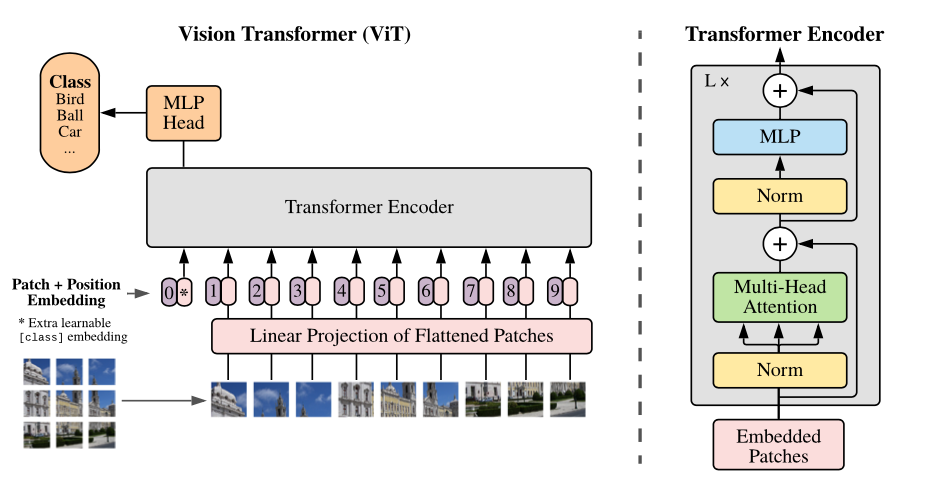
\includegraphics[width=0.88\textwidth]{vit_overview.png}
\caption[Vision Transformer và bộ mã hóa patch]{Minh họa Vision Transformer.\\
\textit{Nguồn:} Google Research \cite{vit}.}\label{fig:vit}
\end{figure}
Điểm này bằng trung bình cosine giữa ảnh và từng prompt. Nếu chuẩn hóa lại $\widetilde
q_c=\unit(q_c)$ thì độ dài prototype không còn ảnh hưởng trực tiếp đến điểm. Hai phép gộp có thể đổi
thứ hạng lớp; vì thế báo cáo tách đối chứng raw mean và unit mean.

\begin{sloppypar}
Bộ mã hóa chính là MetaCLIP2 ViT-H/14 với checkpoint worldwide tương ứng. Tokenizer thực tế là XLM-V, context 77. Prompt lớp quá context bị từ
chối; tiêu đề mẫu có thể bị tokenizer cắt. Bộ tiền xử lý ảnh lấy từ checkpoint, không thay bằng
preprocessing của một backbone khác.
\end{sloppypar}

Hình~\ref{fig:clip} minh họa tiền huấn luyện CLIP và suy luận zero-shot. Đề tài dùng checkpoint có
sẵn, không chạy lại bước tiền huấn luyện.
\begin{figure}[H]\centering
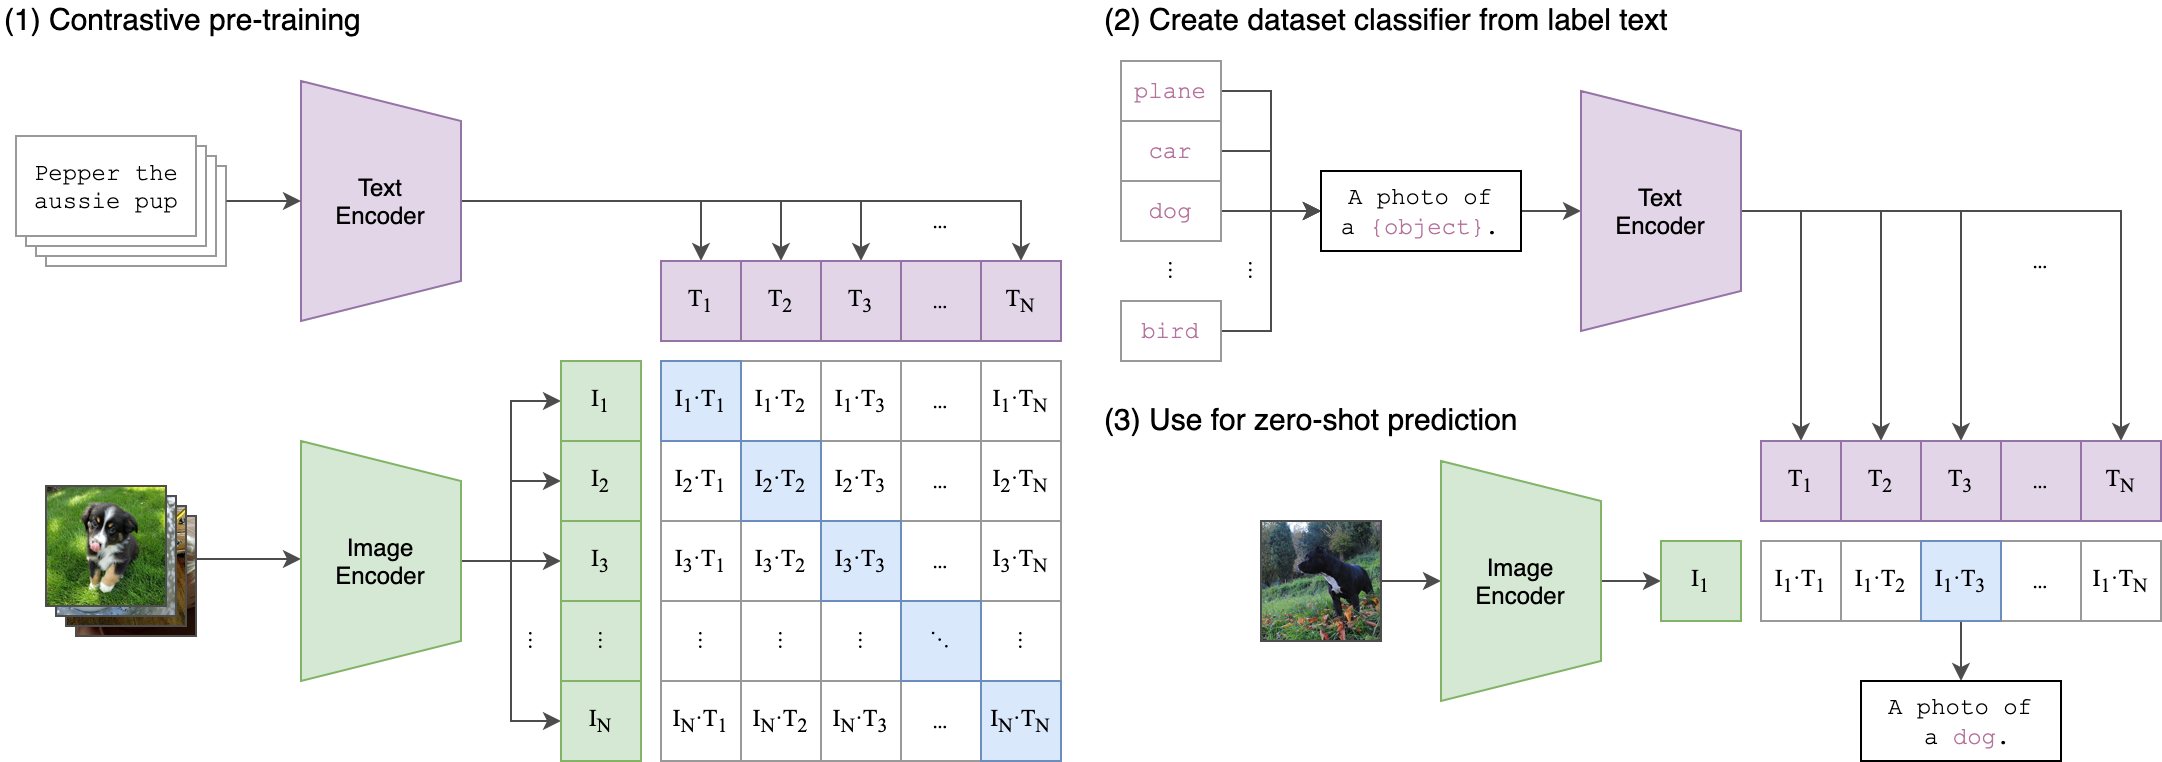
\includegraphics[width=0.95\textwidth]{clip_overview.png}
\caption[Tiền huấn luyện CLIP và phân loại zero-shot]{Tiền huấn luyện tương phản và phân loại zero-shot bằng prompt.\\
\textit{Nguồn:} OpenAI CLIP \cite{clip}.}\label{fig:clip}
\end{figure}

\subsection{Phân loại phẳng và prompt lớp}

Khi có cả ảnh và văn bản, mỗi nhánh cho phân phối lớp $p_I(c\mid I_i)$ và $p_T(c\mid t_i)$. Fusion
xác suất cố định có dạng
\begin{equation}
p(c\mid x_i)=w_Ip_I(c\mid I_i)+(1-w_I)p_T(c\mid t_i),\qquad 0\leq w_I\leq1.
\end{equation}
Đây là baseline phẳng: mọi lớp cạnh tranh cùng lúc. Các đối chứng chỉ ảnh, chỉ văn bản và kết hợp dùng cùng cohort để đo đóng góp của từng phương thức.

Hình~\ref{fig:softmax-fusion} minh họa phép gộp xác suất. Các giá trị số trong hình chỉ giải thích
cách tính, không phải kết quả một lượt chạy.
\begin{figure}[H]\centering
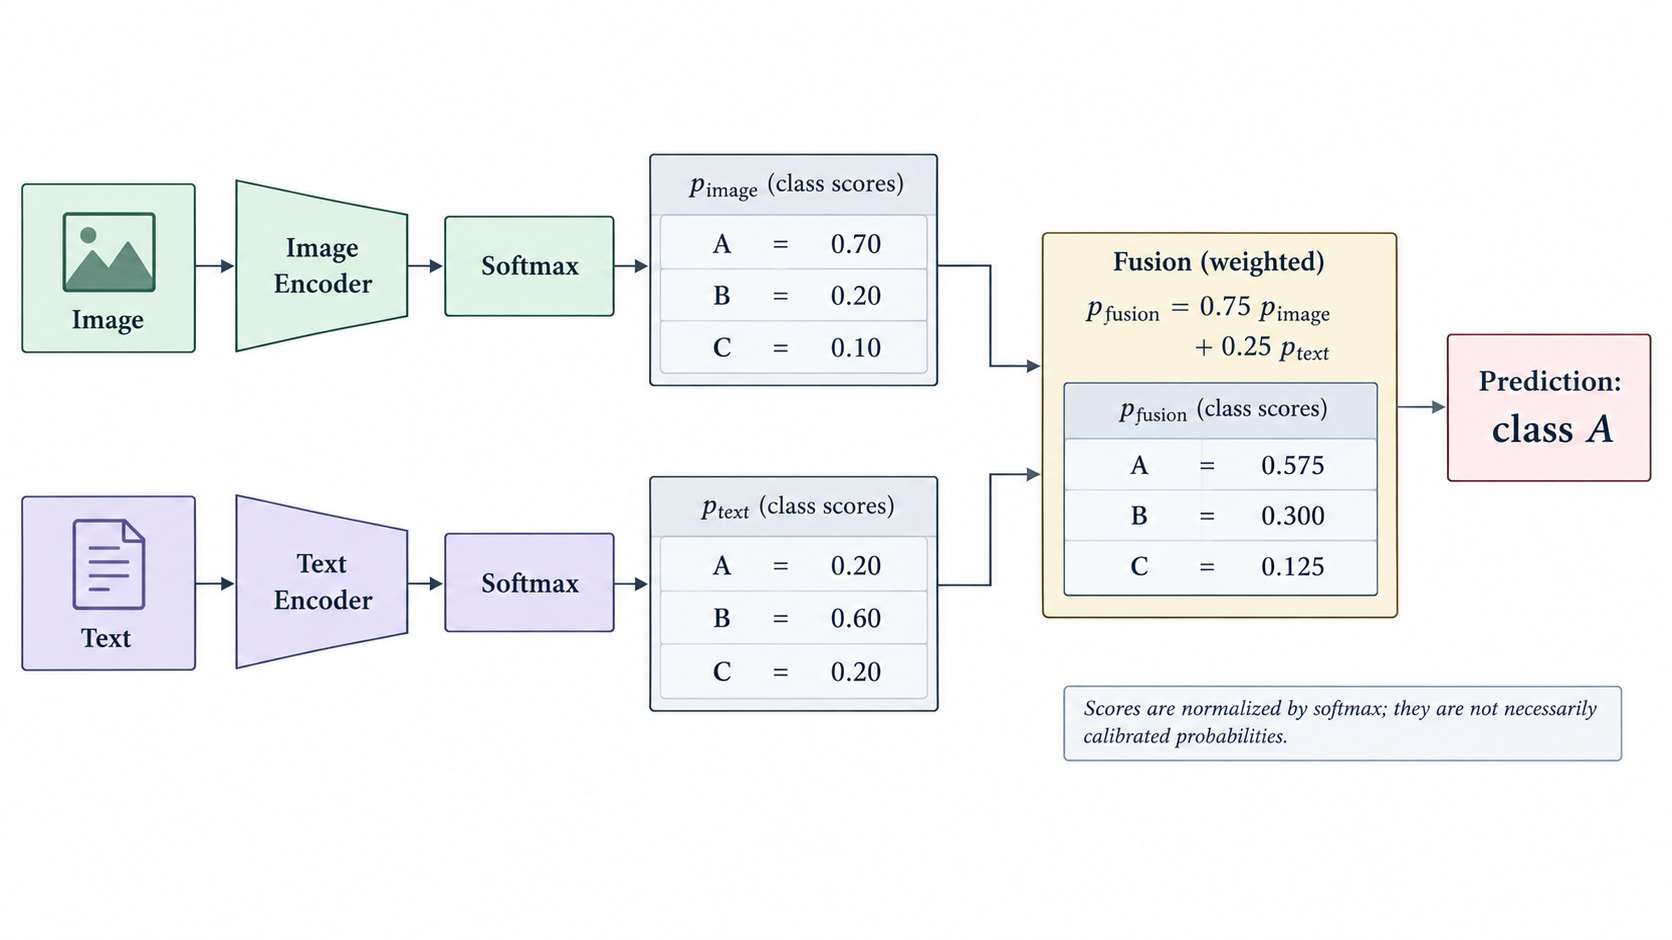
\includegraphics[width=0.94\textwidth]{Soft_max_fusion.png}
\caption{Minh họa fusion có trọng số sau softmax cho phân loại một nhãn. Các điểm trong hình là ví dụ tính toán, không phải metric thực nghiệm.}\label{fig:softmax-fusion}
\end{figure}

\subsubsection{DCLIP: phân loại bằng mô tả đặc trưng}

DCLIP mô tả một lớp bằng nhiều đặc trưng thay vì chỉ tên lớp \cite{dclip}. Với benchmark, dự án dùng
nguồn descriptor và bộ sinh prompt tác giả đã cố định phiên bản. Descriptor Fakeddit là bản thích
nghi theo taxonomy của dự án; không đồng nhất với mô tả GPT-3 nguyên bản.
Hình~\ref{fig:dclip} minh họa khác biệt giữa tên lớp và các descriptor đặc trưng.
\begin{figure}[H]\centering
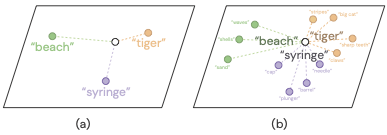
\includegraphics[width=0.68\textwidth]{dclip_descriptors.png}
\caption[Biểu diễn lớp bằng tên lớp và descriptor]{Biểu diễn lớp bằng tên lớp và bằng descriptor.\\
\textit{Nguồn:} Menon và Vondrick \cite{dclip}.}\label{fig:dclip}
\end{figure}

\subsubsection{WaffleCLIP: tổng hợp prompt ngẫu nhiên}

WaffleCLIP thay mô tả ngữ nghĩa bằng các hậu tố từ và ký tự ngẫu nhiên \cite{waffle}. Thiết lập
benchmark dùng 15 cặp, tương ứng 30 prompt mỗi lớp, bảy seed. Không chọn seed tốt nhất. Cần phân
biệt random seed tạo prompt với grouping seed của solver: hai loại seed đo hai nguồn biến thiên khác
nhau.
Hình~\ref{fig:waffle-overview} minh họa ý tưởng tạo nhiều prompt Waffle và so sánh embedding. Phần
hỏi GPT-3 tạo broad concept trong hình là một thành phần của sơ đồ bài báo, không được hiểu là mô hình
được gọi trực tiếp trong từng lượt inference của dự án.
\begin{figure}[H]\centering
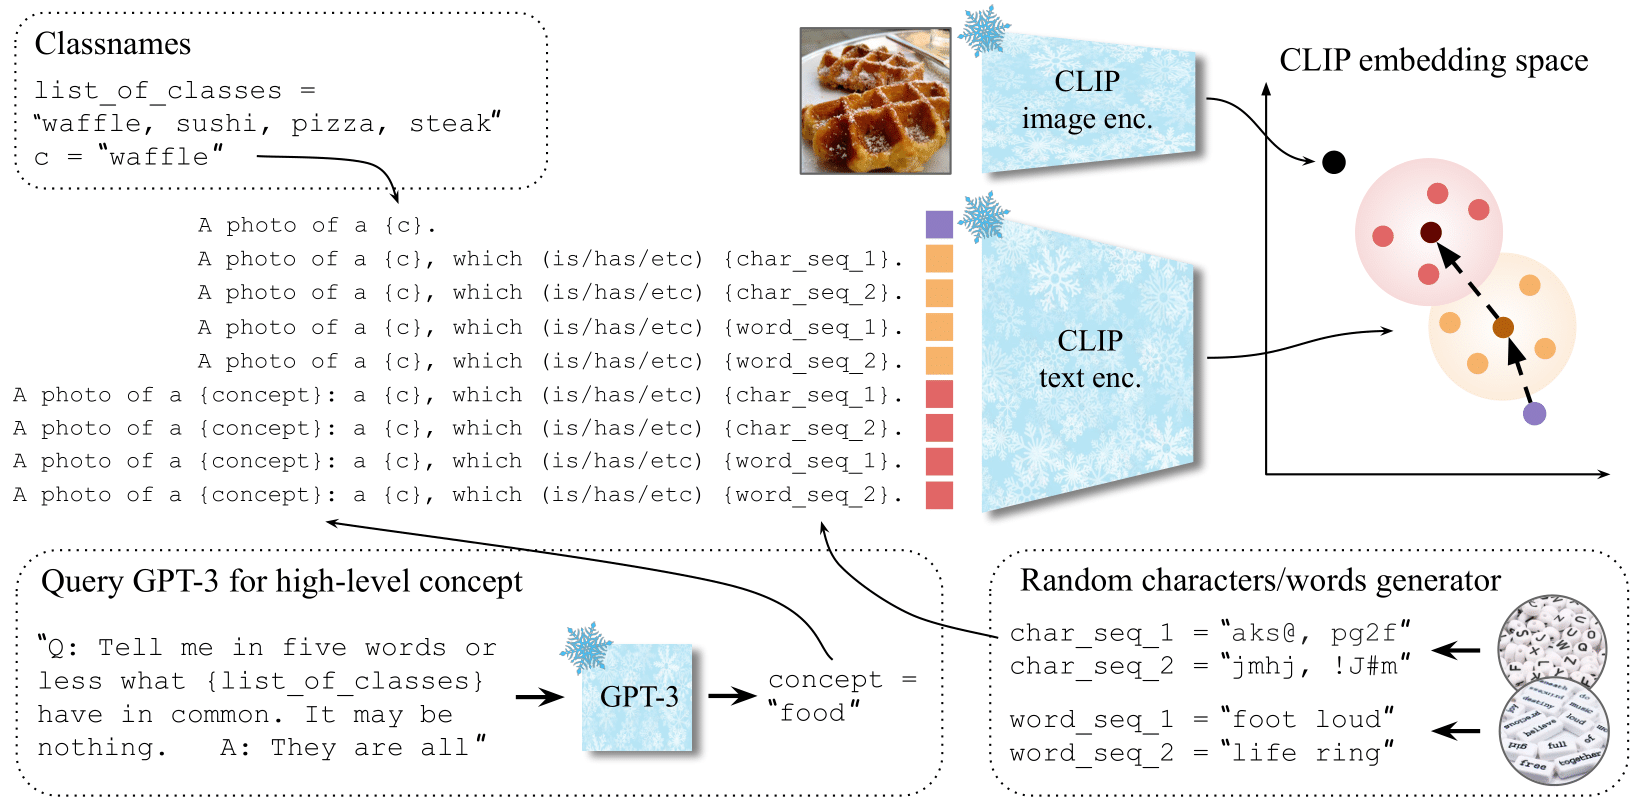
\includegraphics[width=0.96\textwidth]{waffleclip_overview.png}
\caption[WaffleCLIP và các prompt ngẫu nhiên]{Minh họa phương pháp WaffleCLIP: tạo prompt biến thể và tổng hợp biểu diễn lớp.\\
\textit{Nguồn:} Roth và cộng sự \cite{waffle}.}\label{fig:waffle-overview}
\end{figure}


\subsection{Thích nghi không nhãn: inductive và transductive}

\textbf{Inductive zero-shot} dự đoán một mẫu từ encoder và prompt, không cần các query còn lại. \textbf{Transductive zero-shot} sử dụng cấu trúc của một nhóm query không nhãn; dự đoán một ảnh có thể phụ thuộc các ảnh cùng nhóm. EM-Dirichlet là một phương pháp tối ưu trên các vector xác suất ảnh--lớp \cite{em}.

StatA dùng tri thức từ text encoder làm neo thống kê trong thích nghi \cite{stata}. Trong triển khai
dự án, nhóm query tối đa 75 ảnh; grouping seed là 0, 1, 2. Các tham số solver được giữ theo cấu hình
đã triển khai. Tác động của thích nghi được đo riêng trên từng bộ dữ liệu bằng đối chứng có cùng prototype và tập query.

\subsection{Đánh giá trên dữ liệu mất cân bằng}
Accuracy gán trọng số cho từng lớp theo số mẫu thực tế, còn Macro-F1 tổng hợp F1 với trọng số bằng nhau giữa các lớp. Balanced Accuracy (BA) là trung bình Recall theo lớp. Sự khác nhau này giải thích việc thứ hạng hệ thống thay đổi theo chỉ số \cite{metrics}. Trong đối chứng sáu lớp Fakeddit, Macro-F1 là chỉ số chính; Accuracy và BA bổ sung góc nhìn về tổng số mẫu đúng và độ phủ các lớp.

\subsection{Phân loại phân cấp và lỗi định tuyến}

Với nhóm thô $g$ và lớp con $c\in g$, tầng một ước lượng $p(g\mid x)$, tầng hai ước lượng
$p(c\mid g,x)$:
\begin{equation}
p(c\mid x)=p(g_c\mid x)\,p(c\mid g_c,x),
\end{equation}
trong đó $g_c$ là nhóm chứa lớp $c$. Nếu hard gate loại nhóm đúng thì tầng sau không còn lớp đúng
trong tập ứng viên. Vì vậy phải báo cáo metric gate, metric tầng con khi gate đúng và metric
end-to-end. Kết quả oracle dùng nhóm thật chỉ là chẩn đoán.

Fakeddit có cấu trúc Real/Fake rồi tới True hoặc một trong năm loại Fake \cite{fakeddit}; CIFAR-100
có 20 nhóm coarse rồi tới 100 lớp fine. Hai taxonomy cần đánh giá riêng.

\subsection{Few-shot trên embedding đóng băng}

\textbf{Few-shot linear probing} học một bộ phân loại từ support có nhãn train trên embedding đóng băng. Dù encoder không cập nhật, quy trình này vẫn có giám sát và khác zero-shot. Giao thức xác định số support, seed và quy tắc chọn siêu tham số. Nhãn train tham gia học bộ phân loại; nhãn dev tham gia tính chỉ số sau khi đã tạo dự đoán. Điểm few-shot được báo trong các bảng riêng với điểm zero-shot.

\subsection{Chỉ số và cách báo cáo}

Với lớp $c$, các đại lượng cơ bản là
\begin{equation}
P_c=\frac{TP_c}{TP_c+FP_c},\quad R_c=\frac{TP_c}{TP_c+FN_c},\quad
F1_c=\frac{2TP_c}{2TP_c+FP_c+FN_c}.
\end{equation}
Quy ước mẫu số bằng 0 cho giá trị 0. Accuracy đo tỷ lệ mẫu đúng; Macro-F1 và BA lần lượt là trung
bình F1 và Recall trên toàn taxonomy. Benchmark có thêm top-5; không dùng top-5 cho quyết định
binary.

Qua $K$ seed, báo cáo trung bình và sample standard deviation:
\begin{equation}
\bar m=\frac1K\sum_{k=1}^K m_k,\qquad s=\sqrt{\frac{\sum_k(m_k-\bar m)^2}{K-1}}.
\end{equation}
Với phương pháp tất định, báo cáo trình bày giá trị của lượt chạy tương ứng. Độ lệch chuẩn trên cùng cohort không phải
khoảng tin cậy. Các tổ hợp bảy prompt seed với ba grouping seed có chia sẻ dữ liệu và thành phần
ngẫu nhiên, không phải 21 tập đánh giá độc lập.
\newpage


% KẾT THÚC: 09. NỘI DUNG CHƯƠNG 2


% ============================================================================
% 10. NỘI DUNG CHƯƠNG 3
% ============================================================================
\Chapter{PHƯƠNG PHÁP VÀ TRIỂN KHAI}
\subsection{Kiến trúc tổng thể}
Hệ thống tách bộ mã hóa khỏi bộ ra quyết định. Bộ mã hóa chuyển ảnh, tiêu đề và prompt lớp thành vector; bộ ra quyết định sử dụng độ tương đồng, thích nghi không nhãn hoặc bộ phân loại tuyến tính. Cách tổ chức này giữ thống nhất biểu diễn đầu vào trong từng đối chứng và cho phép thay đổi quy tắc quyết định mà vẫn dùng lại các đặc trưng đã mã hóa.

\begin{figure}[H]\centering
\begin{tikzpicture}[font=\BodyFont,>=Latex,box/.style={draw,rounded corners,align=center,text width=4.1cm,minimum height=1.1cm,fill=blue!5},link/.style={->,thick}]
\node[box] (input) at (0,0) {Ảnh và văn bản};
\node[box] (enc) at (0,-1.8) {Bộ mã hóa đóng băng\\đặc trưng chuẩn hóa};
\node[box] (zs) at (-3,-3.9) {Zero-shot\\prompt, prototype, StatA};
\node[box] (fs) at (3,-3.9) {Few-shot\\support train, linear probing};
\node[box] (zout) at (-3,-6) {Quyết định phẳng\\hoặc phân cấp};
\node[box] (fout) at (3,-6) {Real/Fake, phẳng sáu lớp\\hoặc cascade hai tầng};
\draw[link] (input)--(enc);
\draw[link] (enc.south)--++(0,-0.5)-|(zs.north);
\draw[link] (enc.south)--++(0,-0.5)-|(fs.north);
\draw[link] (zs)--(zout);\draw[link] (fs)--(fout);
\end{tikzpicture}
\caption{Các nhánh thực nghiệm dùng biểu diễn thị giác--ngôn ngữ. Mỗi nhánh được đánh giá theo giao thức dữ liệu và nguồn giám sát tương ứng. Sơ đồ do nhóm xây dựng.}
\label{fig:architecture}
\end{figure}

\subsection{Xây dựng và kết hợp prototype lớp}
CLIP dùng prompt tên lớp; DCLIP dùng tập mô tả đặc trưng lớp; Waffle dùng các hậu tố ngẫu nhiên. Với các prompt đã mã hóa và chuẩn hóa, dự án giữ hai phép gộp: trung bình trực tiếp (raw mean) và chuẩn hóa lại vector trung bình (unit mean). Đối chứng này xác định ảnh hưởng của độ dài prototype trước khi phân tích tác dụng của ngữ nghĩa.

Gọi $q_c^W$ là prototype Waffle và $q_c^D$ là prototype mô tả ngữ nghĩa. Biến thể kết hợp có dạng
\begin{equation}
q_c^{WS}=\unit\big((1-\alpha)\unit(q_c^W)+\alpha\unit(q_c^D)\big).
\end{equation}
Hệ số $\alpha=0{,}5$ được giữ cố định trên DTD và EuroSAT. Điểm ảnh--lớp được tính từ tích vô hướng giữa embedding ảnh unit và prototype. Nhánh thích nghi sử dụng prototype kết hợp làm tri thức khởi tạo của StatA. Thiết kế giữ các đối chứng Waffle unit và Waffle--semantic để tách tác động của bước kết hợp khỏi bước thích nghi.

\subsection{Kết hợp ảnh và tiêu đề}
Trong zero-shot, ảnh và tiêu đề được so với cùng bộ mô tả lớp, sau đó gộp phân phối điểm bằng trọng số cố định của từng cấu hình. Hai nhánh ảnh riêng và tiêu đề riêng là đối chứng cho phương thức kết hợp.

Trong few-shot, với hai embedding unit $u_i$ và $v_i$, các đặc trưng được xác định bởi
\begin{equation}
h_I(x_i)=u_i,\qquad h_T(x_i)=v_i,\qquad
h_{IT}(x_i)=\frac{[u_i;v_i]}{\sqrt{2}}.
\end{equation}
Đặc trưng nối $h_{IT}$ có norm bằng 1 vì tổng bình phương norm hai thành phần bằng 2. Logistic Regression học trực tiếp trên đặc trưng này, thay cho việc cộng hai phân phối dự đoán riêng. Mỗi seed, ba phương thức ảnh, tiêu đề và ảnh--tiêu đề dùng cùng support.

Bộ phân loại dùng $C=1$, trọng số lớp cân bằng, solver LBFGS, tối đa 2.000 vòng lặp và ngưỡng dừng $10^{-6}$. Các tham số được học là hệ số và intercept; trọng số encoder giữ nguyên. Với $n_c$ mẫu support của lớp $c$ trong bài toán $K$ lớp, trọng số lớp tương ứng là $w_c=n/(Kn_c)$. Quy tắc này được áp dụng riêng cho từng head theo các lớp mà head học.

\subsection{Ngân sách nhãn và chọn support}
Mỗi seed sử dụng 384 mẫu train. Năm seed là $0,1,2,3,4$. Hai cách phân bổ được ký hiệu nhất quán như sau:
\begin{itemize}
\item \textbf{L (cân bằng sáu lớp):} 64 mẫu mỗi lớp, tương ứng 64 Real và 320 Fake.
\item \textbf{B (cân bằng nhị phân):} 192 Real và 192 Fake; mỗi subtype Fake có 38 mẫu và hai suất dư được luân phiên theo seed.
\end{itemize}
Ký hiệu L tương ứng với tên Legacy trong các bảng nhị phân; B tương ứng với Balanced.
Hai support L và B có chung 256 ID trong từng seed; B thay 128 mẫu Fake bằng 128 mẫu Real. Hợp của mười support gồm 1.591 ID được mã hóa một lần để tiết kiệm tính toán. Mỗi mô hình học từ đúng 384 ID của support tương ứng. Phân bổ B đồng thời tăng độ phủ Real và giảm số mẫu Fake; do trọng số lớp đã cân bằng ở cả hai cách phân bổ, đây là đối chứng về ngân sách mẫu có nhãn.

Nhãn sáu lớp được ánh xạ sang nhãn gate bằng $y_b=\mathbf1[y_6\ne0]$: $0$ là Real và $1$ là Fake. Trong nhãn sáu lớp, chỉ số $0$ là True/Real, các chỉ số $1$--$5$ lần lượt là Satire/Parody, False Connection, Imposter, Manipulated và Misleading. Tên lớp và thứ tự cột dự đoán được cố định trong suốt đánh giá.

\subsection{Phẳng sáu lớp và cascade hai tầng}
Từ mỗi support, hệ thống học ba head trên cùng đặc trưng ảnh--tiêu đề: head phẳng sáu lớp, gate Real/Fake và head năm loại Fake. Gate và head phẳng học trên 384 mẫu; head con học trên các mẫu Fake của chính support đó, gồm 320 mẫu ở L hoặc 192 mẫu ở B. Tổng ngân sách dữ liệu có nhãn của mỗi hệ thống vẫn là 384 mẫu.

Gọi $p_G$ là đầu ra gate và $p_F$ là đầu ra head con. Quyết định hard gate là
\begin{equation}
\widehat y(x)=
\begin{cases}
0,&\widehat g(x)=\mathrm{Real},\\
1+\arg\max_{j\in\{0,\ldots,4\}}p_F(j\mid x),&\widehat g(x)=\mathrm{Fake}.
\end{cases}
\label{eq:hard-route}
\end{equation}
Quy tắc này ra quyết định nhóm trước rồi chọn lớp con trong nhóm Fake. Phép phân rã xác suất ở Chương 2 mô tả quan hệ nhóm--lớp; phương pháp triển khai dùng quyết định cứng trong Công thức~\ref{eq:hard-route}.

\begin{figure}[H]\centering
\begin{tikzpicture}[font=\BodyFont,>=Latex,box/.style={draw,rounded corners,align=center,text width=3.2cm,minimum height=1.05cm,fill=blue!5},link/.style={->,thick}]
\node[box] (f) at (0,0) {Đặc trưng ảnh--tiêu đề\\$h_{IT}(x)$};
\node[box] (g) at (0,-1.9) {Gate nhị phân\\Real / Fake};
\node[box,fill=green!8] (r) at (-3,-4) {Đầu ra Real\\lớp 0};
\node[box] (c) at (3,-4) {Head năm loại Fake};
\node[box,fill=orange!10] (y) at (3,-6) {Một trong năm subtype\\lớp 1--5};
\draw[link] (f)--(g);\draw[link] (g.south)--++(0,-0.5)-|node[pos=.75,left]{Real}(r.north);
\draw[link] (g.south)--++(0,-0.5)-|node[pos=.75,right]{Fake}(c.north);
\draw[link] (c)--(y);
\end{tikzpicture}
\caption{Suy luận hai tầng trên Fakeddit. Gate và head con nhận cùng đặc trưng; đường đi quyết định lớp đầu ra. Sơ đồ do nhóm xây dựng.}
\label{fig:cascade}
\end{figure}

Mỗi cách phân bổ support có hai quy tắc gate. \textbf{Mặc định} dùng argmax nhị phân và chọn Real khi hòa điểm. \textbf{R87} dùng ngưỡng điểm Fake đã được chọn trên phần selection dev với mục tiêu Recall Fake 87\%, rồi giữ nguyên trong đánh giá cascade. Nhãn R87 biểu thị mục tiêu chọn ngưỡng; giá trị Recall thực tế được báo từ dự đoán. Ngưỡng xác suất cụ thể phụ thuộc support và seed.

\subsection{Phân tích lỗi định tuyến}
Trên từng seed, lỗi sáu lớp được chia thành ba nhóm rời nhau:
\begin{equation}
N_{\mathrm{err}}=N_{R\rightarrow F}+N_{F\rightarrow R}
+N_{\mathrm{child}\mid\mathrm{correct\ Fake\ gate}}.
\label{eq:error-decomposition}
\end{equation}
Nhóm thứ nhất gồm Real bị đưa tới head Fake; nhóm thứ hai gồm Fake bị trả về Real; nhóm thứ ba gồm Fake được định tuyến đúng nhưng nhận sai subtype. Phép chia này gắn từng lỗi đầu cuối với vị trí phát sinh trong hệ thống. Với một subtype Fake, Recall đầu cuối bằng tỷ lệ mẫu vừa được gate nhận là Fake vừa được head con phân loại đúng; vì vậy nó bị giới hạn bởi Recall gate của subtype đó.

Đánh giá head con trên toàn bộ Fake thật tách chất lượng head khỏi lựa chọn mẫu của gate. Chẩn đoán oracle thay quyết định gate bằng nhóm thật và giữ nguyên head con, qua đó đo ảnh hưởng của định tuyến đối với số mẫu phân loại đúng. Oracle được trình bày riêng với các phương pháp suy luận.

\subsection{Lưu vết và kiểm tra kết quả}
Mỗi lượt chạy lưu cấu hình, nhận dạng tập mẫu, support theo seed, thứ tự lớp, dự đoán từng ID, chỉ số từng lớp và chỉ số tổng hợp. Các tệp đầu ra có checksum để kiểm tra tính toàn vẹn. Dự đoán được tạo trước khi đối chiếu nhãn dev; các head chỉ học từ nhãn support train.

Ma trận cascade lưu 30 tổ hợp phương pháp--seed và 90.000 dòng dự đoán. Kiểm tra lại từ dự đoán xác nhận Accuracy, Macro-F1, BA và trung bình, độ lệch chuẩn của sáu phương pháp. Phép replay từ đầu ra gate và head con tái tạo đúng nhãn hard route. Gate được kế thừa từ thí nghiệm nhị phân, với mười bộ đầu ra trùng khớp giữa hai ma trận.
\clearpage


% KẾT THÚC: 10. NỘI DUNG CHƯƠNG 3


% ============================================================================
% 11. NỘI DUNG CHƯƠNG 4
% ============================================================================
\Chapter{THIẾT KẾ THỰC NGHIỆM}
\subsection{Dữ liệu và đơn vị đánh giá}
\begin{table}[H]\centering\BodyFont
\caption{Phạm vi dữ liệu thực nghiệm của báo cáo}
\begin{tabularx}{\linewidth}{@{}p{.25\linewidth}p{.20\linewidth}L@{}}\toprule
Nhóm dữ liệu & Quy mô & Phạm vi đánh giá\\\midrule
Tham chiếu OpenAI & 160.093 ảnh & Tám bộ dữ liệu; 88 lượt đánh giá\\
DTD & 1.880 ảnh & 47 lớp, test partition 1\\
ImageNetV2 & 10.000 ảnh & MatchedFrequency, 1.000 lớp\\
EuroSAT & 27.000 ảnh & Toàn bộ ảnh RGB, 10 lớp\\
Fakeddit dev cũ & 3.000 mẫu & 1.537 Real và 1.463 Fake\\
Fakeddit min5 & 3.000 train; 3.000 dev & Dev gồm 1.202 Real và 1.798 Fake\\
CIFAR-100 dev & 10.000 ảnh & 100 lớp fine, 20 nhóm coarse\\\bottomrule
\end{tabularx}\label{tab:datasets}
\end{table}

DTD cung cấp các thuộc tính kết cấu \cite{dtd}; EuroSAT cung cấp các lớp sử dụng đất và lớp phủ bề mặt từ ảnh Sentinel-2 \cite{eurosat}. Trong thí nghiệm này, EuroSAT sử dụng ảnh RGB và bộ tên lớp của giao thức prompt. DTD và EuroSAT được dùng để phát triển các biến thể prototype và thích nghi. Fakeddit dev được dùng cho so sánh phương pháp, phân tích lỗi và lựa chọn cấu hình phát triển.

Cohort Fakeddit min5 dùng ngưỡng độ dài văn bản cấu hình bằng 5 và seed chọn mẫu 42. Dữ liệu học support lấy từ train; dữ liệu tính chỉ số lấy từ dev. Kiểm tra nhận dạng mẫu bao gồm ID, URL, tiêu đề, nội dung ảnh và pixels. Dev cũ và min5 có 2.098 ID chung trên 3.000 mẫu; mỗi phía có 902 ID riêng. Các bảng hai cohort được tách nhãn rõ ràng.

\begin{table}[H]\centering\BodyFont
\caption{Phân bố sáu lớp trên 3.000 mẫu dev Fakeddit min5}
\begin{tabularx}{\linewidth}{@{}Lrr@{}}\toprule
Lớp & Số mẫu & Tỷ lệ (\%)\\\midrule
Real & 1.202 & 40,07\\
Satire/Parody & 182 & 6,07\\
False Connection & 572 & 19,07\\
Imposter & 64 & 2,13\\
Manipulated & 868 & 28,93\\
Misleading & 112 & 3,73\\\midrule
Tổng & 3.000 & 100,00\\\bottomrule
\end{tabularx}\label{tab:class-counts}
\end{table}
Fakeddit sử dụng nhãn được xây dựng bằng giám sát từ xa (distant supervision) \cite{fakeddit}. Đích đánh giá trong báo cáo là phân loại theo hệ nhãn dữ liệu. Các chỉ số mô tả sự phù hợp của dự đoán với nhãn này trên tập mẫu đã xác định.

\subsection{Backbone và cấu hình suy luận}
Nhánh kiểm chứng tham chiếu sử dụng OpenAI CLIP ViT-L/14 ở độ phân giải 224 px. Mỗi bộ dữ liệu có 11 lượt đánh giá, gồm bảy seed Waffle và các đối chứng prompt. Kết quả của nhánh này được trình bày riêng với MetaCLIP2.

Backbone chính là MetaCLIP2 ViT-H/14, với checkpoint, tokenizer và phép tiền xử lý ảnh tương ứng. Các lượt MetaCLIP2 chính dùng CUDA FP32, batch ảnh thông thường bằng 8 và batch prompt bằng 64. Luồng mã hóa prompt hỗ trợ giảm batch 64/32/16 theo bộ nhớ khả dụng và giữ nguyên tập prompt. Runtime và phiên bản thư viện được lưu theo từng lượt chạy.

Waffle dùng bảy seed prompt. Các đối chứng StatA dùng ba grouping seed, nhóm query tối đa 75 ảnh. Với tổ hợp Waffle và StatA, kết quả tổng hợp qua bảy seed prompt và ba seed chia nhóm. Few-shot dùng năm seed support; phép tính độ lệch chuẩn sử dụng mẫu số $K-1$.

\subsection{Ma trận đối chứng và chỉ số chính}
\begin{table}[H]\centering\BodyFont
\caption{Các nhóm đối chứng và yếu tố được kiểm soát}
\begin{tabularx}{\linewidth}{@{}p{.26\linewidth}L@{}}\toprule
Nhóm đối chứng & Thiết kế\\\midrule
Prompt tham chiếu & Cùng OpenAI ViT-L/14, cùng bộ dữ liệu; thay cách mô tả lớp\\
Prototype kết hợp & Cùng MetaCLIP2; tách Waffle unit, Waffle--semantic và thêm StatA\\
Real/Fake zero-shot & Cùng min5 dev; ảnh, tiêu đề, fusion và thích nghi\\
Few-shot nhị phân & Ba modality, hai support L/B, năm seed, 384 nhãn/seed\\
Few-shot sáu lớp & Phẳng, cascade mặc định, cascade R87; hai support L/B; cùng 3.000 ID\\\bottomrule
\end{tabularx}
\end{table}

Trong ma trận sáu lớp, Macro-F1 là chỉ số chính vì các lớp có quy mô chênh lệch rõ rệt, từ 64 mẫu Imposter tới 1.202 mẫu Real. Accuracy phản ánh tổng số mẫu đúng, còn BA phản ánh Recall trung bình theo lớp. Các nhận xét về thứ hạng luôn gắn với chỉ số cụ thể. Báo cáo sử dụng điểm phần trăm để diễn đạt chênh lệch giữa hai tỷ lệ phần trăm.

Đối chứng cascade gồm sáu phương pháp và năm seed, tương ứng 30 tổ hợp, tất cả dùng đặc trưng ảnh--tiêu đề và cùng họ Logistic Regression. Thay đổi giữa phẳng và cascade được tính ghép cặp trong cùng support và seed. Ngưỡng R87 được kế thừa từ selection dev; phần kiểm tra nội bộ gồm 1.500 ID audit dev cố định. Full dev và audit dev cùng thuộc phạm vi đánh giá phát triển.

\subsection{Đối chiếu tham chiếu và tính nhất quán}
Ngưỡng đối chiếu số học của nhánh tham chiếu là sai lệch tuyệt đối tối đa 0,10 điểm phần trăm. Nguồn đối chiếu là các kết quả tác giả và số liệu công bố của CLIP, DCLIP, WaffleCLIP \cite{clip,dclip,waffle}. Báo cáo phân biệt kết quả của nhóm với mốc nguồn và phân biệt sample standard deviation của thí nghiệm với population standard deviation trong bảng tác giả.

Các phép so sánh trực tiếp giữ cùng tập ID, nhãn, backbone và chế độ học. Các đối chứng lịch sử Fakeddit dev cũ và CIFAR-100 được trình bày theo cohort riêng. Thí nghiệm zero-shot, thích nghi không nhãn và few-shot được xác định theo dữ liệu tham gia ra quyết định; nhờ đó các mức Accuracy được diễn giải cùng ngân sách giám sát tương ứng.
\clearpage


% KẾT THÚC: 11. NỘI DUNG CHƯƠNG 4


% ============================================================================
% 12. NỘI DUNG CHƯƠNG 5
% ============================================================================
\Chapter{KẾT QUẢ VÀ PHÂN TÍCH}

\subsection{Kiểm chứng triển khai trên tám bộ dữ liệu ảnh}

\begin{table}[H]

\centering
\BodyFont
\caption{Accuracy tham chiếu OpenAI ViT-L/14 trên tám dataset (\%).}
\begin{tabularx}{\linewidth}{@{}L r r r r r@{}}
\toprule
Dataset & Ảnh & CLIP photo & DCLIP photo & Waffle & Gần khớp\\
\midrule
DTD & 1.880 & 52,98 & 56,22 & 53,82 & 0/3\\
ImageNetV2 & 10.000 & 67,91 & 69,73 & 69,50 & 3/3\\
ImageNet & 50.000 & 73,38 & 75,24 & 75,28 & 3/3\\
CUB & 5.794 & 62,25 & 63,57 & 64,16 & 3/3\\
Food101 & 25.250 & 92,54 & 92,84 & 93,28 & 3/3\\
Pets & 3.669 & 93,19 & 93,89 & 91,92 & 2/3\\
EuroSAT & 27.000 & 56,05 & 58,53 & 61,48 & 1/3\\
Places365 & 36.500 & 40,06 & 42,57 & 42,12 & 1/3\\
\bottomrule
\end{tabularx}
\par\medskip
\begin{minipage}{\linewidth}
    \BodyFont
Waffle là trung bình bảy seed; bảng này chỉ hiển thị mean. Cột cuối là số đối chiếu chính đạt ngưỡng
0,10 điểm phần trăm theo ngưỡng đối chiếu đã xác định; không bao gồm hai đối chứng prompt gốc.
\end{minipage}

\end{table}

Nhánh tham chiếu hoàn tất tám dataset, 160.093 ảnh và 1.761.023 dòng dự đoán. Có 16/24 đối chiếu
chính đạt ngưỡng gần khớp; nếu tính cả hai đối chứng prompt gốc thì có 20/40 đối chiếu số học đạt
ngưỡng. Hoàn tất số lượng ảnh không đồng nghĩa tất cả phép tái lập khớp paper.

ImageNetV2, ImageNet, CUB và Food101 đạt 3/3 đối chiếu chính; DTD đạt 0/3. Pets, EuroSAT và Places365 lần lượt đạt 2/3, 1/3 và 1/3. Các con số thể hiện mức độ gần khớp số học theo cùng ngưỡng đối chiếu; đánh giá này giữ nguyên kết quả đo của nhóm và mốc nguồn.

\subsection{Đối chứng prompt trên MetaCLIP2}

\begin{table}[H]

\centering
\BodyFont
\caption{Các đối chứng prompt chuẩn trên MetaCLIP2 (\%).}
\begin{tabularx}{\linewidth}{@{}L r r r@{}}
\toprule
Dataset / phương pháp & Accuracy & Macro-F1 & Top-5\\
\midrule
DTD / CLIP & 66,76 & 64,39 & 90,59\\
DTD / DCLIP & 64,79 & 62,08 & 92,77\\
DTD / Waffle & 68,94 $\pm$ 0,23 & 66,95 $\pm$ 0,25 & 93,53 $\pm$ 0,25\\
DTD / Waffle unit & 69,59 $\pm$ 0,16 & 67,71 $\pm$ 0,19 & 93,66 $\pm$ 0,12\\
ImageNetV2 / CLIP & 74,00 & 73,54 & 92,92\\
ImageNetV2 / DCLIP & 73,76 & 72,92 & 92,77\\
ImageNetV2 / Waffle & 74,48 $\pm$ 0,12 & 73,95 $\pm$ 0,12 & 93,21 $\pm$ 0,11\\
ImageNetV2 / Waffle unit & 74,29 $\pm$ 0,12 & 73,87 $\pm$ 0,12 & 93,23 $\pm$ 0,11\\
\bottomrule
\end{tabularx}
\par\medskip
\begin{minipage}{\linewidth}
    \BodyFont
Mean $\pm$ sample std qua bảy seed với Waffle; CLIP/DCLIP là một lượt tất định.
\end{minipage}

\end{table}

Trên DTD, Waffle và Waffle unit tốt hơn CLIP; unit tốt hơn Waffle raw mean khoảng 0,65 điểm phần
trăm Accuracy. Trên ImageNetV2, Waffle raw mean lại tốt hơn unit khoảng 0,19 điểm phần trăm. DCLIP
thấp hơn CLIP ở cả hai bộ trong các lượt này. Vì thế, không có cơ sở coi descriptor ngữ nghĩa hoặc
chuẩn hóa prototype là luôn có lợi.

Ma trận prompt chuẩn trên MetaCLIP2 gồm DTD và ImageNetV2. EuroSAT được đánh giá trong ma trận kết hợp semantic--StatA ở mục kế tiếp. Các bảng xác định rõ backbone và dữ liệu của từng đối chứng.

\subsection{Kết hợp Waffle--semantic và StatA}

\begin{table}[H]

    \centering
    \BodyFont
    \caption{Kết hợp prototype và StatA trên DTD (\%).}
    \begin{tabularx}{\linewidth}{@{}L R R@{}}
        \toprule
        Phương pháp & Accuracy & Macro-F1 \\
        \midrule
        CLIP & 66,76 & 64,39 \\
        CLIP--StatA & 66,95 $\pm$ 0,08 & 64,84 $\pm$ 0,22 \\
        Semantic unit & 66,01 & 63,59 \\
        Semantic--StatA & 66,90 $\pm$ 0,13 & 65,15 $\pm$ 0,11 \\
        Waffle & 68,94 $\pm$ 0,23 & 66,95 $\pm$ 0,25 \\
        Waffle unit & 69,59 $\pm$ 0,16 & 67,71 $\pm$ 0,19 \\
        Waffle--StatA & 69,25 $\pm$ 0,33 & 67,78 $\pm$ 0,38 \\
        Waffle--semantic & 70,40 $\pm$ 0,23 & 68,65 $\pm$ 0,26 \\
        Waffle--semantic--StatA & 71,10 $\pm$ 0,24 & 69,95 $\pm$ 0,23 \\
        \bottomrule
    \end{tabularx}
    \par\medskip
    \begin{minipage}{\linewidth}
        \BodyFont
Waffle dùng bảy prompt seed; StatA dùng ba grouping seed;
nhánh kết hợp dùng 21 tổ hợp. Giá trị sau dấu $\pm$ là sample std.
    
\end{minipage}

\end{table}

\begin{table}[H]

    \centering
    \BodyFont
    \caption{Kết hợp prototype và StatA trên EuroSAT (\%).}
    \begin{tabularx}{\linewidth}{@{}L R R@{}}
        \toprule
        Phương pháp & Accuracy & Macro-F1 \\
        \midrule
        CLIP & 64,06 & 62,13 \\
        CLIP--StatA & 60,69 $\pm$ 0,04 & 53,97 $\pm$ 0,06 \\
        Semantic unit & 57,20 & 55,21 \\
        Semantic--StatA & 57,78 $\pm$ 0,06 & 55,68 $\pm$ 0,05 \\
        Waffle & 62,66 $\pm$ 0,59 & 62,01 $\pm$ 0,96 \\
        Waffle unit & 62,95 $\pm$ 0,52 & 61,01 $\pm$ 0,70 \\
        Waffle--StatA & 60,25 $\pm$ 0,59 & 53,77 $\pm$ 0,50 \\
        Waffle--semantic & 64,42 $\pm$ 0,41 & 64,08 $\pm$ 0,48 \\
        Waffle--semantic--StatA & 61,73 $\pm$ 0,50 & 57,13 $\pm$ 0,64 \\
        \bottomrule
    \end{tabularx}
    \par\medskip
    \begin{minipage}{\linewidth}
        \BodyFont
Waffle dùng bảy prompt seed; StatA dùng ba grouping seed;
nhánh kết hợp dùng 21 tổ hợp. Giá trị sau dấu $\pm$ là sample std.
    
\end{minipage}

\end{table}

Trên DTD, kết hợp Waffle--semantic--StatA đạt Accuracy 71,10\%, tăng 4,34 điểm phần trăm so CLIP,
1,51 so Waffle unit và khoảng 0,69 so Waffle--semantic. Trong 21 đối chiếu cùng prompt/grouping
seed, nhánh ba thành phần đều hơn Waffle--semantic về Accuracy. Tuy nhiên, top-5 giảm từ 94,95\%
xuống 93,11\%; phương pháp không tốt hơn trên mọi chỉ số.

Trên EuroSAT, Waffle--semantic không StatA đạt Accuracy 64,42\%, Macro-F1 64,08\%, cao hơn CLIP lần
lượt khoảng 0,36 và 1,95 điểm phần trăm. Thêm StatA làm Accuracy giảm 2,69 điểm phần trăm và thua cả
21 đối chiếu ghép cặp. Recall annual crop land giảm từ 30,98\% xuống 0,88\%, brushland/shrubland từ
17,19\% xuống 0,89\%; một số lớp khác tăng. Các thay đổi Recall cho thấy mức giảm tổng thể đi kèm sự dịch chuyển mạnh của dự đoán giữa các lớp.

\begin{figure}[H]

    \centering
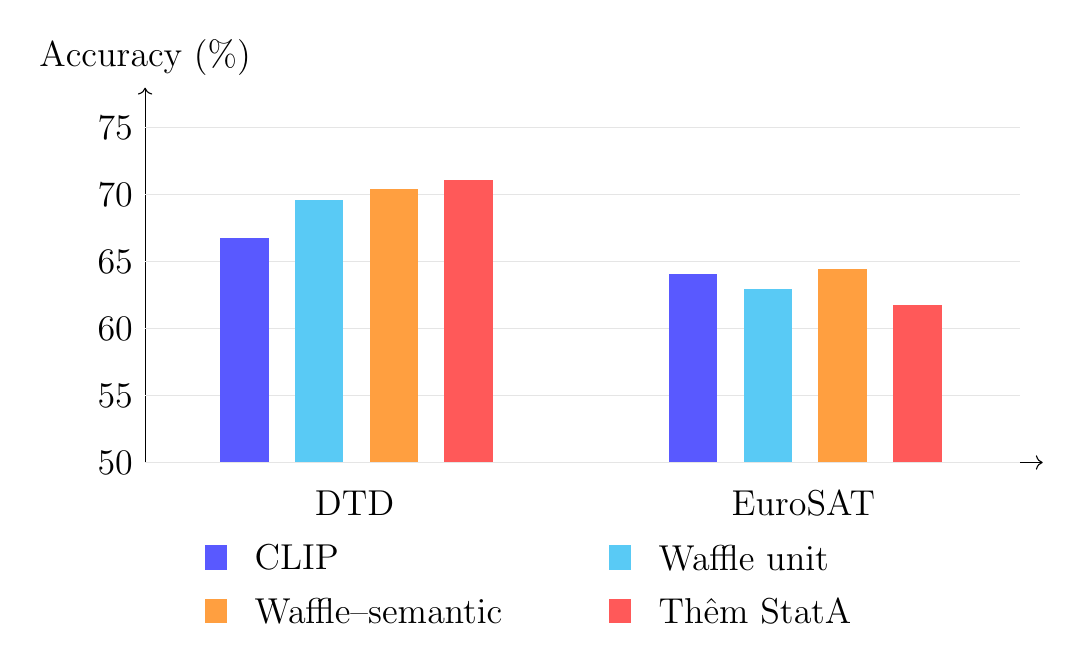
\begin{tikzpicture}[x=0.95cm,y=0.17cm,font=\BodyFont]
    \draw[->] (0,0) -- (0,28) node[above]{Accuracy (\%)};
    \draw[->] (0,0) -- (12,0);

    \foreach \value in {50,55,60,65,70,75} {
        \pgfmathsetmacro{\height}{\value-50}
        \draw[gray!20] (0,\height) -- (11.7,\height);
        \node[left] at (0,\height) {\value};
    }

    \foreach \position/\value/\colour in {
        1/66.7553/blue!65,
        2/69.5897/cyan!65,
        3/70.4027/orange!75,
        4/71.0968/red!65,
        7/64.0593/blue!65,
        8/62.9540/cyan!65,
        9/64.4228/orange!75,
        10/61.7328/red!65
    } {
        \pgfmathsetmacro{\height}{\value-50}
        \fill[\colour] (\position,0) rectangle +(0.65,\height);
    }

    \node[below] at (2.8,-1.2) {DTD};
    \node[below] at (8.8,-1.2) {EuroSAT};

    % Hai dòng chú giải, tránh tên phương pháp chạm nhau.
    \fill[blue!65] (0.8,-8) rectangle +(0.3,1.8);
    \node[anchor=west] at (1.3,-7.1) {CLIP};

    \fill[cyan!65] (6.2,-8) rectangle +(0.3,1.8);
    \node[anchor=west] at (6.7,-7.1) {Waffle unit};

    \fill[orange!75] (0.8,-12) rectangle +(0.3,1.8);
    \node[anchor=west] at (1.3,-11.1) {Waffle--semantic};

    \fill[red!65] (6.2,-12) rectangle +(0.3,1.8);
    \node[anchor=west] at (6.7,-11.1) {Thêm StatA};
\end{tikzpicture}
\caption{So sánh phương pháp trên cùng full cohort của từng dataset. Trục tung bắt đầu từ 50\%; giá trị cột là trung bình seed khi phương pháp có nhiều seed.}

\end{figure}

Kết quả hai miền ủng hộ tiếp tục kiểm chứng Waffle--semantic không StatA như ứng viên chuyển miền.
Chưa đủ bằng chứng chọn nhánh ba thành phần làm mặc định chung. Tín hiệu Waffle--StatA pilot 256 ảnh
DTD đạt 72,32\% không được dùng thay số full: trên đủ DTD, Waffle--StatA chỉ đạt 69,25\%, thấp hơn
Waffle unit 69,59\%.

\subsection{Fakeddit Real/Fake zero-shot trên dev min5}

\begin{table}[H]

\centering
\BodyFont
\caption{Fakeddit 2way không dùng nhãn train trên dev min5 (\%).}
\begin{tabularx}{\linewidth}{@{}L r r r@{}}
\toprule
Phương pháp & Accuracy & Macro-F1 & BA\\
\midrule
CLIP ảnh & 63,87 & 63,03 & 63,37\\
CLIP tiêu đề & 57,50 & 56,66 & 56,99\\
CLIP ảnh--tiêu đề & 64,07 & 63,27 & 63,65\\
StatA ảnh & 72,02 $\pm$ 0,27 & 71,29 $\pm$ 0,32 & 71,69 $\pm$ 0,38\\
CLIP--StatA ảnh & 71,26 $\pm$ 0,32 & 70,54 $\pm$ 0,35 & 70,96 $\pm$ 0,38\\
CLIP--StatA ảnh--tiêu đề & 71,17 $\pm$ 0,39 & 70,46 $\pm$ 0,42 & 70,89 $\pm$ 0,46\\
\bottomrule
\end{tabularx}
\par\medskip
\begin{minipage}{\linewidth}
    \BodyFont
Mỗi lượt đủ 3.000 dev. Các nhánh StatA dùng ba grouping seed; các baseline CLIP tất định một lượt.
\end{minipage}

\end{table}

StatA ảnh riêng đạt Accuracy 72,02\%, Macro-F1 71,29\% và BA 71,69\%, tốt nhất trong sáu đối chứng
không dùng nhãn train. Nhánh CLIP--StatA ảnh--tiêu đề tốt hơn CLIP ảnh--tiêu đề nhưng thấp hơn StatA
ảnh khoảng 0,86 điểm phần trăm Accuracy. Đối chứng này ghi nhận StatA ảnh đạt mức Accuracy cao hơn công thức fusion ảnh--tiêu đề được khảo sát.

Quy tắc luôn chọn Fake đạt Accuracy 59,93\% và BA 50\%; cần đọc đồng thời Macro-F1/BA để tránh chỉ
nhìn lớp đông. Kết quả StatA 65,88\% trên dev cũ và 72,02\% trên min5 thuộc hai cohort khác nhau,
không dùng mức chênh đó để kết luận giảm ngưỡng văn bản cải thiện thuật toán.

\subsection{Đối chứng phân cấp trên các cohort bổ sung}

Trên Fakeddit dev cũ, hierarchy StatA image-only đạt Accuracy 50,36\% và Macro-F1 31,34\%, so flat
StatA 39,63\% và 29,27\%. Original hierarchy Majority đa phương thức đạt 50,33\% và 31,37\%, so
legacy flat đa phương thức 35,60\% và 26,24\%. Tuy nhiên, Accuracy vẫn thấp hơn 51,23\% của quy tắc
luôn chọn True; Macro-F1 của quy tắc đó chỉ 11,29\%. Không kết luận chất lượng tuyệt đối tốt chỉ vì
vượt flat hiện có.

Thêm CALIP sau cùng gate StatA ở nhánh đa phương thức tăng Macro-F1 từ 31,57\% lên 31,74\% nhưng
giảm Accuracy từ 50,27\% xuống 50,16\%. Phân tích bootstrap ghép cặp đã lưu cho delta Macro-F1 có
khoảng 95\% $[-0{,}2247;\,0{,}6847]$ điểm phần trăm, chứa 0. Hai chỉ số thay đổi theo hướng khác nhau và khoảng bootstrap chứa 0; mức thay đổi Macro-F1 được diễn giải theo phạm vi này.

Trên CIFAR-100 dev 10.000 ảnh, flat tên lớp đạt Accuracy 86,75\%; hai tầng cứng và mềm chỉ đạt
58,10\% và 67,19\%. Nhánh coarse trực tiếp đạt 63,44\%, cho thấy rủi ro định tuyến. Đối chứng flat
dùng mô tả đạt 88,38\%, còn top-2 nhóm dùng cùng mô tả đạt 88,10\%. Lợi ích quan sát được đến từ
thay mô tả; lọc nhóm đạt Accuracy thấp hơn đối chứng phẳng cùng mô tả. Các nhánh flat EM, StatA và Majority lần lượt đạt
64,66\%, 86,01\% và 86,44\%, đều không vượt flat CLIP trong lượt này.

Các con số oracle dùng nhóm hoặc gate thật chỉ phục vụ chẩn đoán, không được đưa vào bảng thành tích
mô hình. Kết quả CIFAR và Fakeddit khác nhau nhấn mạnh vai trò taxonomy và khả năng của router.

\subsection{Few-shot Real/Fake và phân bổ support}

\begin{table}[H]

\centering
\BodyFont
\caption{Few-shot với cùng 384 support mỗi seed trên dev min5 (\%).}
\begin{tabularx}{\linewidth}{@{}L r r r@{}}
\toprule
Modality (Real/Fake) & Accuracy & Macro-F1 & BA\\
\midrule
Ảnh (64/320) & 77,83 $\pm$ 1,07 & 76,91 $\pm$ 1,20 & 76,91 $\pm$ 1,30\\
Tiêu đề (64/320) & 77,17 $\pm$ 0,75 & 75,43 $\pm$ 1,14 & 74,88 $\pm$ 1,30\\
Ảnh--tiêu đề (64/320) & 81,22 $\pm$ 0,75 & 80,16 $\pm$ 0,88 & 79,81 $\pm$ 1,02\\
Ảnh (192/192) & 79,93 $\pm$ 0,63 & 79,64 $\pm$ 0,62 & 80,77 $\pm$ 0,60\\
Tiêu đề (192/192) & 78,66 $\pm$ 0,57 & 77,95 $\pm$ 0,63 & 78,21 $\pm$ 0,76\\
Ảnh--tiêu đề (192/192) & 82,41 $\pm$ 0,47 & 82,04 $\pm$ 0,43 & 82,87 $\pm$ 0,36\\
\bottomrule
\end{tabularx}
\par\medskip
\begin{minipage}{\linewidth}
    \BodyFont
Năm seed support 0--4, cùng 3.000 dev; encoder đóng băng, Logistic Regression C=1. Hai policy có
cùng tổng ngân sách và khác phân bổ Real/Fake.
\end{minipage}

\end{table}

Với legacy support 64 Real/320 Fake, kết hợp ảnh--tiêu đề đạt Accuracy 81,22\%, hơn ảnh riêng 3,39
điểm phần trăm và tiêu đề riêng 4,05 điểm phần trăm. Chênh lệch Accuracy so hai nhánh riêng dương ở
cả năm seed trên cùng support và cohort. Đây là bằng chứng văn bản bổ trợ ảnh trong linear probing
hiện tại, khác với kết quả prompt fusion zero-shot.

Với support 192/192, nhánh kết hợp đạt Accuracy 82,41\%, Macro-F1 82,04\% và BA 82,87\%. So legacy
cùng modality, tăng Accuracy khoảng 1,19 điểm phần trăm, Macro-F1 khoảng 1,89 và BA khoảng 3,06. Đây
là kết quả phát triển tốt nhất về ba chỉ số tổng trong đối chứng support này; không phải kết quả
zero-shot.

\begin{table}[H]

    \centering
    \BodyFont
\caption{Đánh đổi khi cân bằng support của nhánh ảnh--tiêu đề trên dev min5}
\begin{tabularx}{\linewidth}{@{}L r r@{}}
\toprule
Chỉ số trung bình & 64 Real/320 Fake & 192 Real/192 Fake\\
\midrule
Recall Real (\%) & 72,71 & 85,21\\
Recall Fake (\%) & 86,91 & 80,53\\
Real bị nhận thành Fake (mẫu/seed) & 328,0 & 177,8\\
Fake bị nhận thành Real (mẫu/seed) & 235,4 & 350,0\\
\bottomrule
\end{tabularx}

\end{table}

Nhánh balanced giảm trung bình 150,2 lỗi Real mỗi seed nhưng thêm 114,6 lỗi bỏ sót Fake, lợi ích
ròng 35,6 mẫu đúng. Mọi seed đều tăng Recall Real và giảm Recall Fake. Nhận định ``cân bằng support
tốt hơn'' vì thế phải đi kèm mục tiêu đánh đổi.

\begin{table}[H]

    \centering
    \BodyFont
\caption{Tỷ lệ phát hiện Fake theo subtype thật; không phải phân loại đúng subtype}
\begin{tabularx}{\linewidth}{@{}L r r r@{}}
\toprule
Subtype & Số mẫu dev & Legacy (\%) & Balanced (\%)\\
\midrule
Satire/Parody &182&80,77&74,51\\
False Connection &572&71,22&56,08\\
Imposter &64&71,25&59,06\\
Manipulated &868&99,54&99,52\\
Misleading &112&88,04&80,36\\
\bottomrule
\end{tabularx}

\end{table}

False Connection có mức giảm Recall gate lớn nhất trong các subtype được khảo sát. Support B phục hồi Recall Real, còn support L giữ Recall Fake cao hơn. Sự thay đổi này giải thích việc tăng Accuracy nhị phân đi kèm một đánh đổi theo lớp; phần cascade tiếp theo đo ảnh hưởng đó lên quyết định sáu lớp.

\subsection{Phân tích lỗi và đối chứng regularization}

Ở baseline legacy ảnh--tiêu đề, có 264 mẫu sai ở cả năm seed: 151 Real, 81 False Connection, 15
Satire, 10 Imposter, 5 Misleading và 2 Manipulated. Đây là số đếm từ phân tích ID dự đoán đã lưu,
không phải các ví dụ ảnh được xem lại trong báo cáo.

Đối chứng train-only CV giữ support 384 mẫu, thử $C\in\{0{,}01;0{,}1;1;10;100\}$ và ba fold phân
tầng theo nhãn 6way của support train. Chọn $C$ theo BA binary trong train-CV rồi refit support;
không dùng nhãn dev để fit hoặc chọn $C$. Kết quả Accuracy 80,23\%, Macro-F1 78,98\%, thấp hơn
baseline $C=1$ đạt 81,22\% và 80,16\%. Không thay runner gốc bằng đối chứng không cải thiện.

Đối chứng CV và phân bổ support thuộc cùng quá trình nghiên cứu trên dev. Phép fit và chọn $C$ của đối chứng CV sử dụng support train; nhãn dev được dùng để đo kết quả sau khi hoàn tất dự đoán.

\subsection{Few-shot sáu lớp trên cùng Fakeddit min5 dev}
\begin{table}[H]\centering\BodyFont
\caption{Kết quả sáu lớp trên 3.000 mẫu dev: trung bình $\pm$ độ lệch chuẩn mẫu qua năm seed (\%)}
\begin{tabularx}{\linewidth}{@{}Lrrr@{}}\toprule
Phương pháp & Accuracy & Macro-F1 & BA\\\midrule
L -- phẳng & $70,19\pm1,46$ & $60,35\pm1,79$ & $68,62\pm1,17$\\
L -- cascade mặc định & $74,35\pm1,09$ & $62,42\pm1,61$ & $68,22\pm1,11$\\
L -- cascade R87 & $74,60\pm1,33$ & $62,61\pm1,73$ & $68,11\pm1,12$\\
B -- phẳng & $74,07\pm1,29$ & $\mathbf{62,84\pm1,15}$ & $67,97\pm0,89$\\
B -- cascade mặc định & $\mathbf{76,22\pm0,50}$ & $62,49\pm0,98$ & $65,26\pm1,05$\\
B -- cascade R87 & $74,70\pm1,01$ & $62,31\pm1,38$ & $68,15\pm0,74$\\\bottomrule
\end{tabularx}\label{tab:cascade-main}
\par\smallskip\begin{minipage}{\linewidth}\BodyFont L: 64 Real/320 Fake; B: 192 Real/192 Fake. Tất cả head dùng cùng đặc trưng ảnh--tiêu đề. In đậm đánh dấu giá trị trung bình cao nhất của Accuracy và Macro-F1. R87 là mục tiêu chọn ngưỡng trên selection dev.\end{minipage}
\end{table}

Cascade L tăng Accuracy từ 70,19\% lên 74,35\% với gate mặc định và 74,60\% với R87. Macro-F1 tương ứng tăng từ 60,35\% lên 62,42\% và 62,61\%. Mức tăng Accuracy và Macro-F1 so với phẳng L xuất hiện ở cả năm seed. Như vậy, phân cấp có lợi trong đối chứng cùng support L, với BA trung bình giảm nhẹ.

Với support B, cascade mặc định đạt Accuracy cao nhất, 76,22\%, tăng 2,15 điểm phần trăm so với phẳng B. Macro-F1 giảm 0,35 điểm phần trăm và BA giảm 2,71 điểm phần trăm. Phẳng B đạt Macro-F1 trung bình cao nhất trong sáu phương pháp, 62,84\%, hơn cascade L--R87 khoảng 0,23 điểm phần trăm. Các thứ hạng này mô tả giá trị trung bình trên dev; độ lệch chuẩn phản ánh biến thiên support qua năm seed.

\begin{figure}[H]\centering
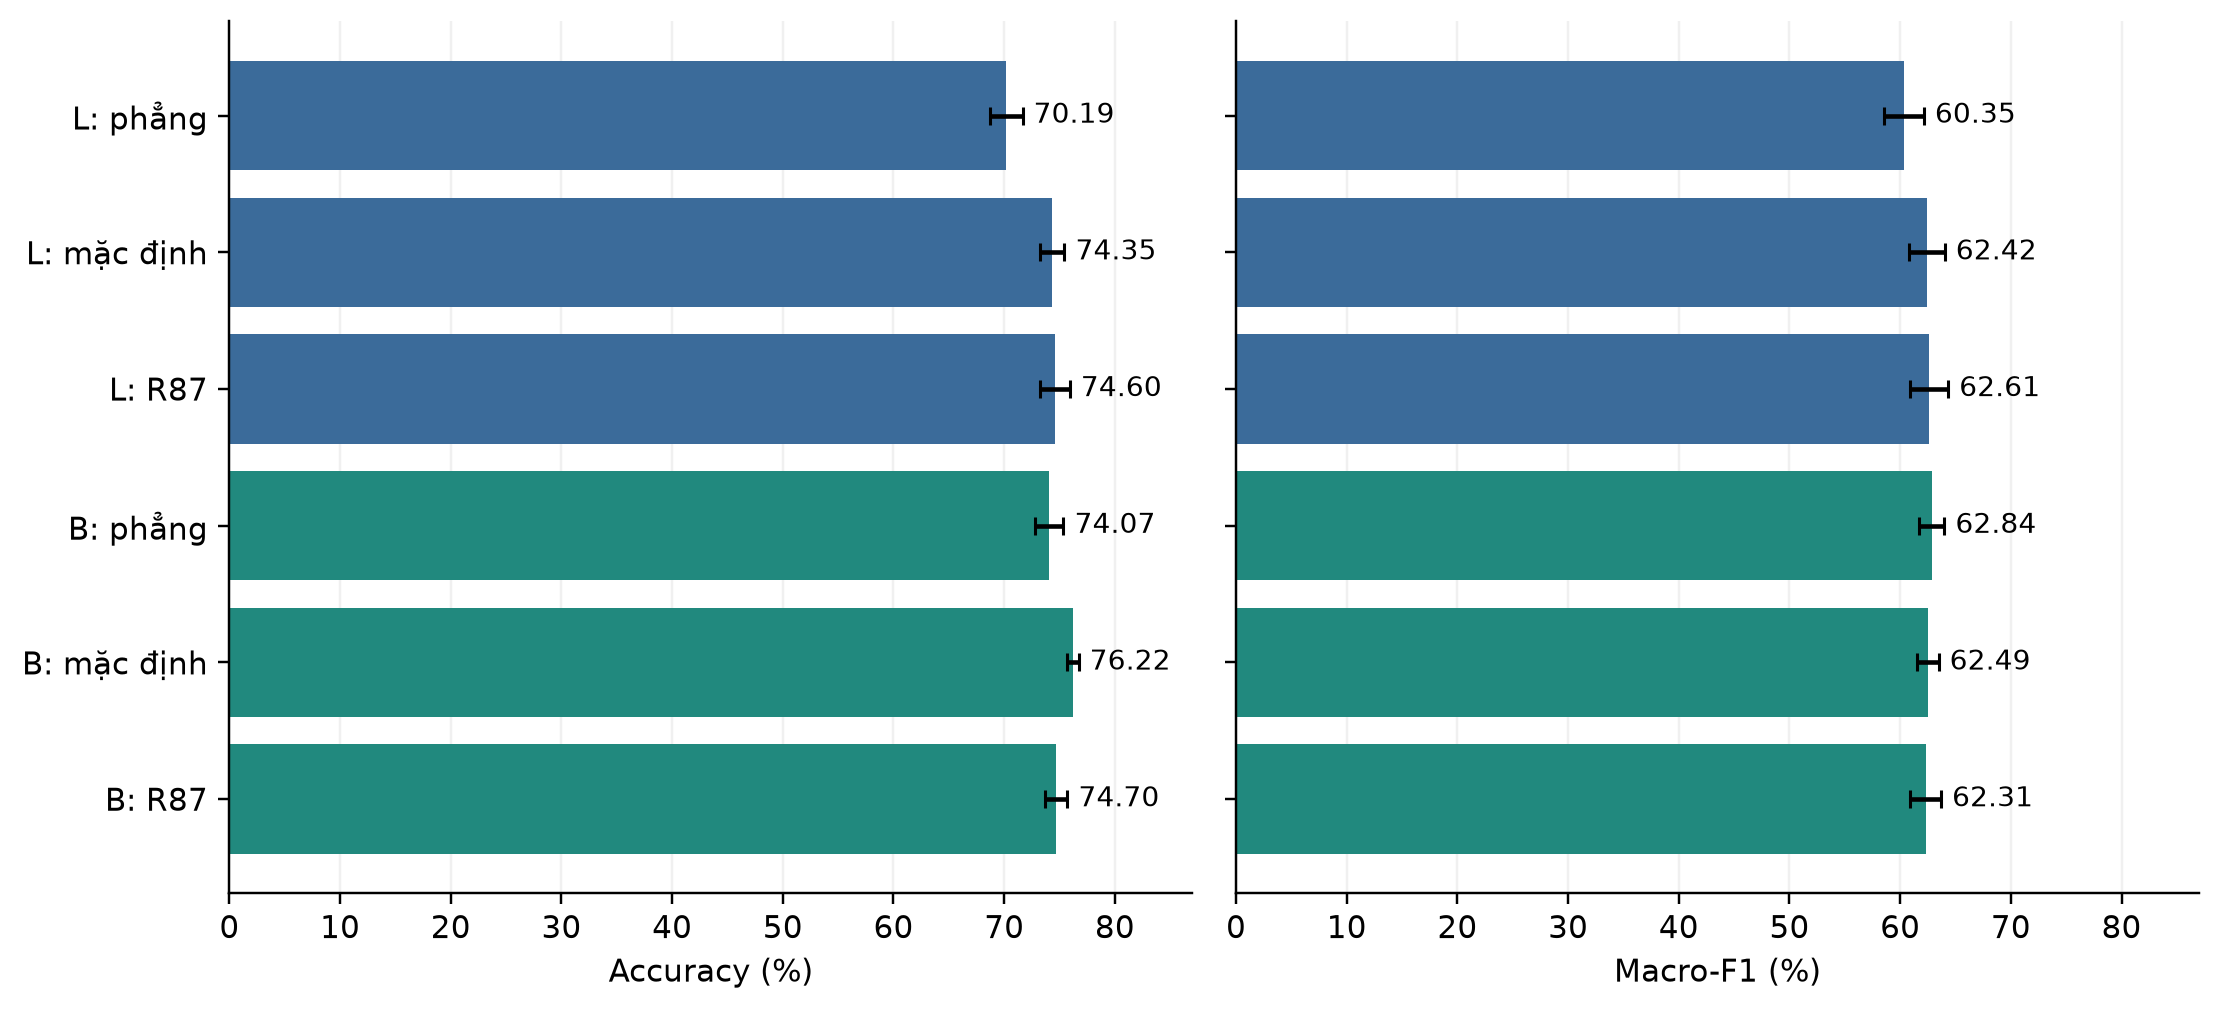
\includegraphics[width=\linewidth]{cascade_metrics.png}
\caption{Accuracy và Macro-F1 của sáu phương pháp trên cùng dev min5. Thanh sai số biểu thị độ lệch chuẩn mẫu qua năm seed. L và B là hai cách phân bổ support. Biểu đồ được dựng từ kết quả thực nghiệm của nhóm.}\label{fig:cascade-metrics}
\end{figure}

\begin{table}[H]\centering\BodyFont
\caption{Chênh lệch ghép cặp giữa cascade và mô hình phẳng cùng support (điểm phần trăm)}
\begin{tabularx}{\linewidth}{@{}Lrrr@{}}\toprule
Cascade so với phẳng & $\Delta$ Accuracy & $\Delta$ Macro-F1 & $\Delta$ BA\\\midrule
L -- mặc định & $+4,16$ & $+2,07$ & $-0,39$\\
L -- R87 & $+4,41$ & $+2,26$ & $-0,50$\\
B -- mặc định & $+2,15$ & $-0,35$ & $-2,71$\\
B -- R87 & $+0,63$ & $-0,53$ & $+0,18$\\\bottomrule
\end{tabularx}
\end{table}
Giữ nguyên ngân sách 384 nhãn nhưng thay support làm thay đổi cả chất lượng gate và số mẫu học head con. L cung cấp 320 mẫu Fake cho head con, còn B cung cấp 192 mẫu. Kết quả vì vậy được diễn giải theo toàn bộ thiết kế phân bổ support và cấu trúc ra quyết định.

\subsection{Gate, head con và phân rã lỗi}
\begin{table}[H]\centering\BodyFont
\caption{Chất lượng gate trên full dev min5, trung bình qua năm seed (\%)}
\begin{tabularx}{\linewidth}{@{}Lrrr@{}}\toprule
Gate & Accuracy nhị phân & Recall Real & Recall Fake\\\midrule
L -- mặc định & 81,22 & 72,71 & 86,91\\
L -- R87 & 81,38 & 73,89 & 86,38\\
B -- mặc định & 82,41 & 85,21 & 80,53\\
B -- R87 & 82,11 & 75,39 & 86,60\\\bottomrule
\end{tabularx}\label{tab:gate-cascade}
\end{table}
Ở B, chuyển từ mặc định sang R87 tăng Recall Fake từ 80,53\% lên 86,60\% và giảm Recall Real từ 85,21\% xuống 75,39\%. Recall mục tiêu 87\% được dùng khi chọn ngưỡng trên selection dev; Recall 86,60\% là kết quả đo trên toàn dev. Sự khác nhau giữa hai giá trị phản ánh đúng hai tập mẫu tham gia chọn ngưỡng và tính chỉ số.

Head con đo trên toàn bộ 1.798 Fake thật đạt Accuracy 84,63\%, Macro-F1 71,13\% ở L; B đạt 83,55\% và 69,88\%. Đây là bài toán năm lớp, được đánh giá trên cùng tập Fake thật với mọi gate. Chỉ số này tách khả năng phân biệt subtype khỏi bước định tuyến.

\begin{table}[H]\centering\BodyFont
\caption{Số lỗi đầu cuối trung bình mỗi seed trên 3.000 mẫu dev}
\begin{tabularx}{\linewidth}{@{}Lrrrr@{}}\toprule
Cascade & Real$\to$Fake & Fake$\to$Real & Sai subtype & Tổng lỗi\\\midrule
L -- mặc định & 328,0 & 235,4 & 206,0 & 769,4\\
L -- R87 & 313,8 & 244,8 & 203,4 & 762,0\\
B -- mặc định & 177,8 & 350,0 & 185,6 & 713,4\\
B -- R87 & 295,8 & 241,0 & 222,2 & 759,0\\\bottomrule
\end{tabularx}\label{tab:routing-errors}
\par\smallskip\begin{minipage}{\linewidth}\BodyFont Sai subtype chỉ tính trên Fake được gate nhận đúng là Fake. Ba nhóm lỗi rời nhau và cộng đúng tổng lỗi đầu cuối.\end{minipage}
\end{table}

Tổng hai nhóm lỗi gate chiếm khoảng 71--74\% lỗi đầu cuối. B--mặc định giảm mạnh số Real bị nhận thành Fake nhưng tăng số Fake trả về Real; kết quả là Accuracy tổng cao hơn trong khi Macro-F1 thấp hơn phẳng B. Phân rã này xác định rõ đóng góp của gate vào kết quả sáu lớp.

\begin{figure}[H]\centering
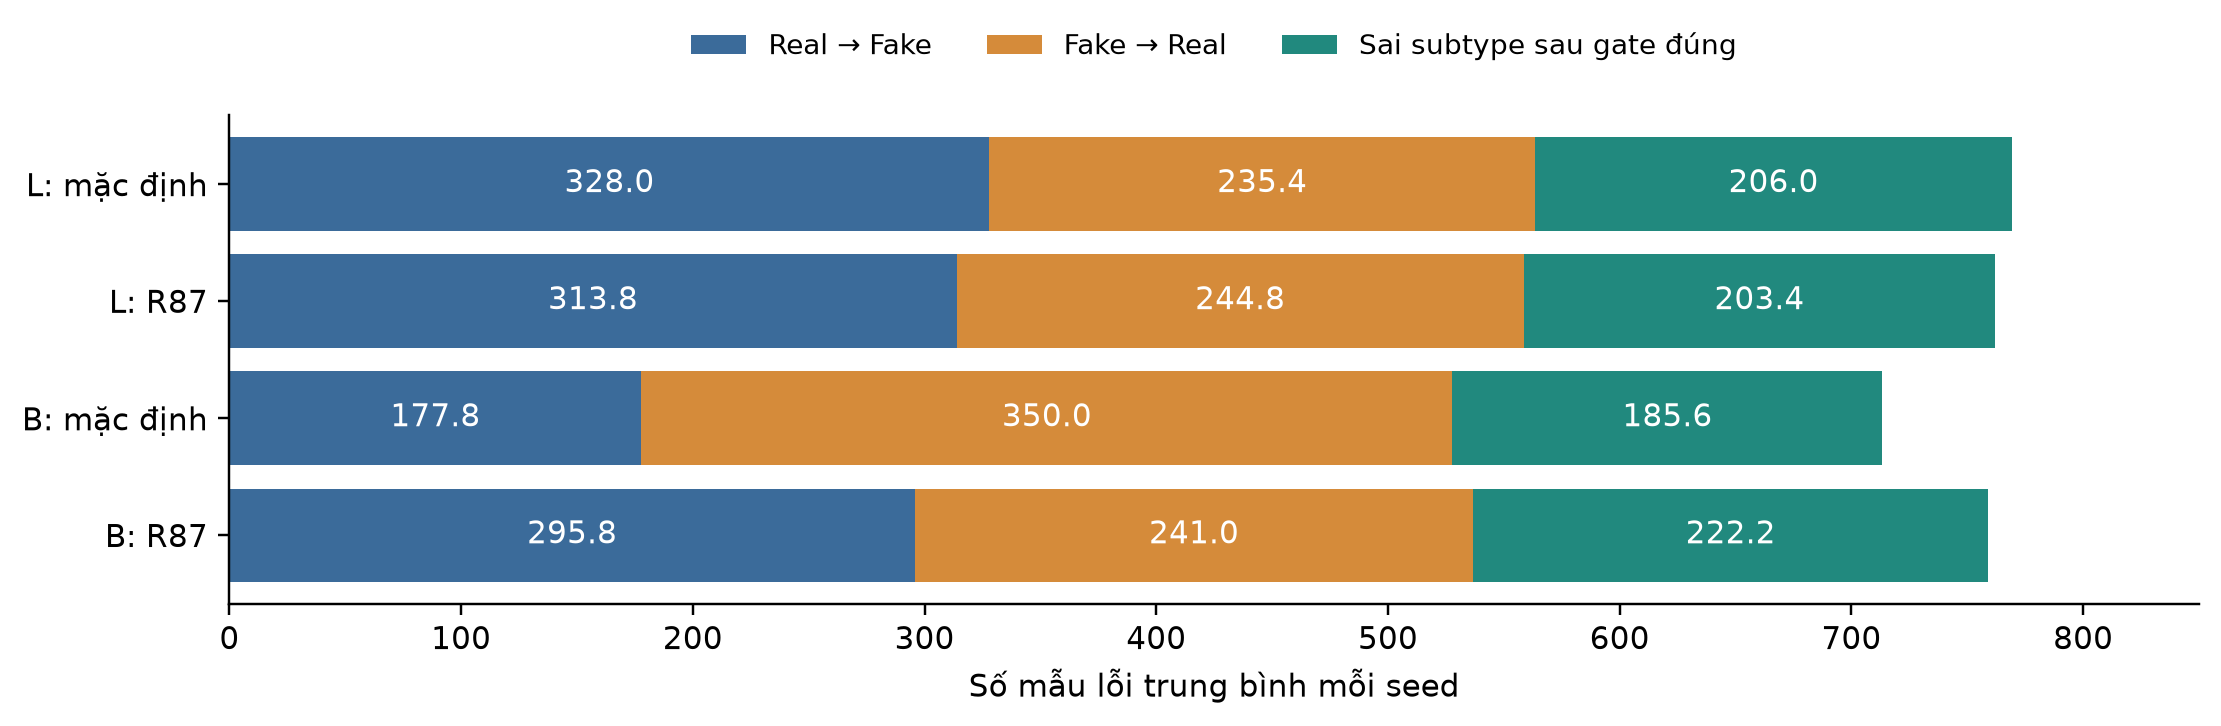
\includegraphics[width=\linewidth]{cascade_errors.png}
\caption{Phân rã lỗi sáu lớp theo vị trí phát sinh, trung bình năm seed. Tổng chiều dài mỗi thanh bằng tổng lỗi của phương pháp tương ứng. Biểu đồ từ thực nghiệm của nhóm.}\label{fig:routing-errors}
\end{figure}

Trong chẩn đoán oracle, dùng nhóm Real/Fake thật và giữ nguyên head con cho Accuracy sáu lớp 90,79\% ở L và 90,14\% ở B. Oracle đo ảnh hưởng của gate khi cố định head con; kết quả được tách khỏi bảng phương pháp suy luận để giữ đúng vai trò chẩn đoán.

\subsection{Kết quả theo subtype và kiểm tra nội bộ}
\begin{table}[H]\centering\BodyFont
\caption{Recall sáu lớp đầu cuối, trung bình năm seed (\%)}
\begin{tabularx}{\linewidth}{@{}Lrrrr@{}}\toprule
Lớp & L mặc định & L R87 & B mặc định & B R87\\\midrule
Real & 72,71 & 73,89 & 85,21 & 75,39\\
Satire/Parody & 63,74 & 63,63 & 59,89 & 63,30\\
False Connection & 47,13 & 46,12 & 33,74 & 43,01\\
Imposter & 49,06 & 49,06 & 41,88 & 50,00\\
Manipulated & 98,11 & 98,11 & 98,18 & 98,29\\
Misleading & 78,57 & 77,86 & 72,68 & 78,93\\\bottomrule
\end{tabularx}\label{tab:subtype-cascade}
\end{table}

Manipulated có Recall khoảng 98\% ở cả bốn cascade. False Connection và Imposter có Recall thấp hơn rõ rệt; ở B--mặc định, False Connection đạt 33,74\%. Với B--R87, Recall lớp này tăng lên 43,01\%, đi kèm sự giảm Recall Real. Sự chênh lệch theo lớp giải thích vì sao Accuracy và Macro-F1 dẫn tới hai thứ hạng khác nhau.

\begin{table}[H]\centering\BodyFont
\caption{Kiểm tra trên 1.500 ID audit dev cố định, trung bình năm seed (\%)}
\begin{tabularx}{\linewidth}{@{}Lrrr@{}}\toprule
Phương pháp & Accuracy & Macro-F1 & BA\\\midrule
L -- phẳng & 70,45 & 60,23 & 68,26\\
L -- cascade mặc định & 74,65 & 62,55 & 68,39\\
L -- cascade R87 & 74,83 & 62,63 & 68,29\\
B -- phẳng & 74,56 & 62,85 & 67,52\\
B -- cascade mặc định & 76,03 & 61,77 & 64,36\\
B -- cascade R87 & 74,77 & 62,08 & 67,94\\\bottomrule
\end{tabularx}\label{tab:audit-cascade}
\end{table}

Phần audit sử dụng cùng 1.500 ID cho mọi phương pháp và giữ nguyên ngưỡng đã chọn. Phẳng B tiếp tục có Macro-F1 cao nhất, 62,85\%; cascade B--mặc định có Accuracy cao nhất, 76,03\%. Kết quả kiểm tra nội bộ này giữ cùng thứ hạng nổi bật với bảng full dev.

\clearpage

% KẾT THÚC: 12. NỘI DUNG CHƯƠNG 5


% ============================================================================
% 13. NỘI DUNG CHƯƠNG 6
% ============================================================================
\Chapter{THẢO LUẬN VÀ KẾT LUẬN}
\subsection{Tác động của mô tả lớp và thích nghi}
Kết quả prompt cho thấy cách biểu diễn lớp là một thành phần thực nghiệm có ảnh hưởng đo được. Trên DTD, chuẩn hóa Waffle prototype tăng Accuracy từ 68,94\% lên 69,59\%; kết hợp semantic và StatA đạt 71,10\%. Trên EuroSAT, Waffle--semantic đạt 64,42\%, còn thêm StatA đạt 61,73\%. Hai miền dữ liệu thể hiện hai tác động khác nhau của cùng hướng thích nghi. Do đó, đánh giá từng thành phần cùng đối chứng cố định là cơ sở của kết luận về phương pháp.

Nhánh tham chiếu hoàn tất tám bộ dữ liệu với 16/24 đối chiếu chính nằm trong ngưỡng sai lệch 0,10 điểm phần trăm. Mức gần khớp này mô tả trực tiếp độ nhất quán của triển khai với các mốc đã chọn. Những đối chiếu nằm ngoài ngưỡng được giữ nguyên trong bảng, giúp kết quả kiểm chứng phản ánh đầy đủ hành vi của hệ thống.

\subsection{Vai trò của ảnh, tiêu đề và ngân sách nhãn}
Trong Real/Fake zero-shot min5, StatA ảnh đạt Accuracy 72,02\%, cao hơn các công thức fusion ảnh--tiêu đề được khảo sát. Trong few-shot L, đặc trưng nối ảnh--tiêu đề đạt 81,22\%, cao hơn ảnh riêng 3,39 điểm phần trăm và tiêu đề riêng 4,05 điểm phần trăm. Như vậy, lợi ích từ văn bản gắn với cách khai thác biểu diễn: học bộ ra quyết định trên đặc trưng nối cho kết quả khác với gộp điểm prompt.

Khi giữ 384 support, chuyển từ L sang B tăng Accuracy nhị phân lên 82,41\% và Macro-F1 lên 82,04\%. Cùng thay đổi đó tăng Recall Real từ 72,71\% lên 85,21\% và giảm Recall Fake từ 86,91\% xuống 80,53\%. Các chỉ số tổng và chỉ số lớp cùng mô tả tác động của phân bổ ngân sách. Kết quả của B phản ánh sự thay đổi thành phần support trong điều kiện trọng số lớp đã cân bằng ở cả hai chính sách.

\subsection{Hiệu quả và đánh đổi của cấu trúc hai tầng}
Trên cùng support L, cascade tăng Accuracy và Macro-F1 so với phẳng ở cả năm seed. Trên support B, cascade mặc định tăng Accuracy nhưng giảm Macro-F1. Trong sáu đối chứng, phẳng B đạt Macro-F1 trung bình cao nhất, 62,84\%, còn cascade B--mặc định đạt Accuracy cao nhất, 76,22\%. Với Macro-F1 là tiêu chí chính của ma trận sáu lớp, phẳng B là mốc đối chứng có giá trị trung bình cao nhất; cascade L--R87 là nhánh phân cấp có Macro-F1 cao nhất, 62,61\%.

Phân rã lỗi cho thấy khoảng 71--74\% lỗi cascade thuộc bước định tuyến. Recall subtype phụ thuộc đồng thời vào khả năng gate nhận diện Fake và khả năng head con phân biệt đúng loại Fake. Kết quả oracle và đánh giá head con trên toàn bộ Fake thật bổ sung hai góc nhìn tách biệt cho mối phụ thuộc này. Phân tích theo lớp cũng chỉ ra chênh lệch lớn giữa Manipulated với False Connection và Imposter, phù hợp với yêu cầu đọc Macro-F1 cùng Accuracy.

\subsection{Phạm vi diễn giải kết quả}
Các kết luận định lượng gắn với backbone, cohort, ngân sách nhãn và quy tắc suy luận của từng bảng. Fakeddit min5 được đánh giá trên tập phát triển; DTD và EuroSAT tham gia phát triển các biến thể prototype và thích nghi. Kiểm tra audit dev là phép đối chiếu nội bộ trên tập con cố định. Độ lệch chuẩn giữa seed biểu thị biến thiên của prompt, cách chia nhóm hoặc support trên cùng tập mẫu, tùy thiết lập; các thanh sai số được diễn giải theo đúng nguồn biến thiên này.

Đối với Fakeddit, hệ thống phân loại theo nhãn distant supervision của dữ liệu. Khái niệm Real/Fake trong báo cáo được sử dụng theo hệ nhãn đó. Báo cáo phân biệt kết quả nhị phân với kết quả sáu lớp, và phân biệt phép chẩn đoán dùng nhóm thật với suy luận dùng gate dự đoán. Những phân biệt này duy trì ý nghĩa nhất quán của từng con số.

\subsection{Kết luận}
Đề tài xây dựng được quy trình phân loại dựa trên mô hình thị giác--ngôn ngữ, gồm prompt zero-shot, kết hợp prototype, thích nghi không nhãn và few-shot trên embedding đóng băng. Thực nghiệm hoàn tất nhánh tham chiếu tám bộ dữ liệu ảnh, các đối chứng MetaCLIP2 trên DTD, ImageNetV2, EuroSAT và các bài toán Fakeddit min5 nhị phân, sáu lớp.

Các kết quả chính gồm Accuracy 71,10\% của Waffle--semantic--StatA trên DTD, 64,42\% của Waffle--semantic trên EuroSAT, và Accuracy 82,41\% cùng Macro-F1 82,04\% của few-shot ảnh--tiêu đề ở bài toán Real/Fake dev min5. Trên sáu lớp của cùng dev, phẳng B đạt Macro-F1 62,84\%, còn cascade B--mặc định đạt Accuracy 76,22\%. Giá trị của đề tài nằm ở việc đo rõ tác dụng từng thành phần, xác định đánh đổi theo lớp và giải thích kết quả đầu cuối bằng lỗi định tuyến trên cùng một giao thức có lưu vết.
\clearpage


% KẾT THÚC: 13. NỘI DUNG CHƯƠNG 6


% ============================================================================
% 14. TÀI LIỆU THAM KHẢO
% ============================================================================
\clearpage
\frontsection{TÀI LIỆU THAM KHẢO}
\begingroup
\BodyFont
\renewcommand{\section}[2]{}
\begin{thebibliography}{99}
\bibitem{clip}
A. Radford và cộng sự, ``Learning Transferable Visual Models From Natural Language Supervision,'' \textit{Proceedings of ICML}, PMLR, tập 139, tr. 8748--8763, 2021.
\url{https://proceedings.mlr.press/v139/radford21a.html}.

\bibitem{vit}
A. Dosovitskiy và cộng sự, ``An Image is Worth 16x16 Words: Transformers for Image Recognition at Scale,'' \textit{ICLR}, 2021.
\url{https://arxiv.org/abs/2010.11929}.

\bibitem{metaclip}
Y.-S. Chuang và cộng sự, ``Meta CLIP 2: A Worldwide Scaling Recipe,'' \textit{arXiv:2507.22062}, 2025.
\url{https://arxiv.org/abs/2507.22062}.

\bibitem{dclip}
S. Menon và C. Vondrick, ``Visual Classification via Description from Large Language Models,'' \textit{ICLR}, 2023.
\url{https://arxiv.org/abs/2210.07183}.

\bibitem{waffle}
K. Roth, J. M. Kim, A. S. Koepke, O. Vinyals, C. Schmid và Z. Akata, ``Waffling around for Performance: Visual Classification with Random Words and Broad Concepts,'' \textit{ICCV}, 2023.
\url{https://arxiv.org/abs/2306.07282}.

\bibitem{em}
S. Martin, Y. Huang, F. Shakeri, J.-C. Pesquet và I. Ben Ayed, ``Transductive Zero-Shot and Few-Shot CLIP,'' \textit{CVPR}, 2024.
\url{https://arxiv.org/abs/2405.18437}.

\bibitem{stata}
M. Zanella, C. Fuchs, C. De Vleeschouwer và I. Ben Ayed, ``Realistic Test-Time Adaptation of Vision-Language Models,'' \textit{arXiv:2501.03729}, 2025.
\url{https://arxiv.org/abs/2501.03729}.

\bibitem{fakeddit}
K. Nakamura, S. Levy và W. Y. Wang, ``Fakeddit: A New Multimodal Benchmark Dataset for Fine-grained Fake News Detection,'' \textit{Proceedings of LREC}, tr. 6149--6157, 2020.
\url{https://aclanthology.org/2020.lrec-1.755/}.

\bibitem{crisis}
F. Alam, F. Ofli và M. Imran, ``CrisisMMD: Multimodal Twitter Datasets from Natural Disasters,'' \textit{ICWSM}, 2018.
\url{https://arxiv.org/abs/1805.00713}.

\bibitem{mmimdb}
J. Arevalo, T. Solorio, M. Montes-y-Gómez và F. A. González, ``Gated Multimodal Units for Information Fusion,'' \textit{arXiv:1702.01992}, 2017.
\url{https://arxiv.org/abs/1702.01992}.

\bibitem{hierarchy}
C. N. Silla Jr. và A. A. Freitas, ``A survey of hierarchical classification across different application domains,'' \textit{Data Mining and Knowledge Discovery}, tập 22, tr. 31--72, 2011.
\url{https://doi.org/10.1007/s10618-010-0175-9}.

\bibitem{metrics}
J. Opitz, ``A Closer Look at Classification Evaluation Metrics and a Critical Reflection of Common Evaluation Practice,'' \textit{Transactions of the Association for Computational Linguistics}, tập 12, tr. 820--836, 2024.
\url{https://aclanthology.org/2024.tacl-1.46/}.

\bibitem{dtd}
M. Cimpoi, S. Maji, I. Kokkinos, S. Mohamed và A. Vedaldi, ``Describing Textures in the Wild,'' \textit{CVPR}, 2014.
\url{https://openaccess.thecvf.com/content_cvpr_2014/html/Cimpoi_Describing_Textures_in_2014_CVPR_paper.html}.

\bibitem{eurosat}
P. Helber, B. Bischke, A. Dengel và D. Borth, ``EuroSAT: A Novel Dataset and Deep Learning Benchmark for Land Use and Land Cover Classification,'' \textit{IEEE Journal of Selected Topics in Applied Earth Observations and Remote Sensing}, 2019.
\url{https://arxiv.org/abs/1709.00029}.
\end{thebibliography}
\endgroup

% KẾT THÚC: 14. TÀI LIỆU THAM KHẢO

\end{document}
